\documentclass{article}
\usepackage{epsfig}
\usepackage{hyperref}
\renewcommand{\baselinestretch}{1}
\setlength{\textheight}{9in}
\setlength{\textwidth}{6.5in}
\setlength{\headheight}{0in}
\setlength{\headsep}{0in}
\setlength{\topmargin}{0in}
\setlength{\oddsidemargin}{0in}
\setlength{\evensidemargin}{0in}
\setlength{\parindent}{.3in}

\usepackage{graphicx}
\graphicspath{ {./images/} }

\usepackage{multicol}
\setlength{\columnseprule}{0em}
\usepackage{listings}

\lstset{
  language=SQL,
  basicstyle=\scriptsize,
  breaklines=true
  }
	
\author{Eduard-Valentin Dumitrescul}
\title{Proiect SGBD - Liga de baschet}
	
\begin{document}

\maketitle

\pagebreak
\tableofcontents
\pagebreak

\section{Prezentare baza de date}
	Prezentați pe scurt baza de date (utilitatea ei).
\subsection{Descrierea Modelului}
	În cadrul unei ligi masculine de baschet, 16 echipe iau parte la fiecare sezon, ce se desfășoară pe parcursul unui an . Fiecare sezon este format din mai multe etape ce se joacă săptămânal, astfel încât până la final, fiecare echipa să fi jucat cu toate celelalte câte două meciuri (acasă și în deplasare). 
	Fiecare echipa este formată din cel puțin 5 jucători, un antrenor, un preparator fizic și un nutriționist. Fiecare echipa deține arena proprie dintr-un anumit oraș, unde va juca meciurile acasă. Pe tot parcursul sezonului se rețin statisticile jucătorilor (puncte marcare, coșuri de 2 puncte, coșuri de 3 puncte, aruncări libere, recuperări, faulturi, pase decisive, apariții) aferente fiecărei etape astfel încât la final să se calculeze clasamentul echipelor și să se acorde diverse premii individuale (pentru cele mai multe puncte marcate, cele mai multe recuperări , cele mai multe pase decisive). La fiecare meci există 3 arbitrii, 3 comentatori și o echipa medicală .

\subsection{Constrângeri}
\begin{itemize}
	\item Într -un moment cel mult un sezon poate fi în curs de desfășurare 
	\item Un sezon conține 30 de etape (pentru a permite echipelor să joace fiecare cu fiecare de exact 2 ori) 
	\item La un sezon iau parte 16 echipe de baschet
	 \item O etapă se desfășoară pe parcursul unei săptămâni calendaristice, iar o singur ă etapă se poate desfășura într -o săptămâna 
	\item O etapă conține 8 meciuri (pentru că fiecare echipa să joace câte un meci). 
	\item Fiecare echipa joacă exact un meci în fiecare etapă . 
	\item Meciul este jucat între două echipe, arena uneia dintre ele. Echipa ce deține arena este considerată că joacă acasă , iar cealaltă în deplasare. 
	\item Un meci nu se poate termină dacă cele două echipe au număr egal de puncte. 
	\item La organizarea fiecărui meci iau parte 3 arbitrii, 3 comentatori și o echipa medicală . 
	\item Fiecare echipa este formată din minim 5 jucători , un antrenor, un preparator fizic, un nutriționist . Nerespectarea minimului de 5 jucători duce la descalificare și la pierderea tuturor meciurilor. 
	\item Fiecare echipa deține o arena aflat într -o locație , iar o arena aparține unei singure echipe. 
	\item Un arbitru, comentator sau echipa medicală pot lua parte la un singur meci la moment dat . 
	\item Un jucător , antrenor, preparator fizic sau nutriționist paote fi angajat de către o singur ă echipa la un moment dat .
	 \item Statisticile sunt realizate la fiecare etapă și sunt păstrate în mod individual,pentru fiecare jucător . 
	\item Premiile individuale sunt acordate unui singur jucător
	
\end{itemize}
\pagebreak
\section{Diagrama Entitate-Relație}
	Realizați diagrama entitate-relație (ERD): entitățile, relațiile și atributele trebuie definite în limba
	română (vezi curs SGBD / model de diagrama ERD; nu se va accepta alt format).


\begin{center}

	\vspace{1cm}
	
	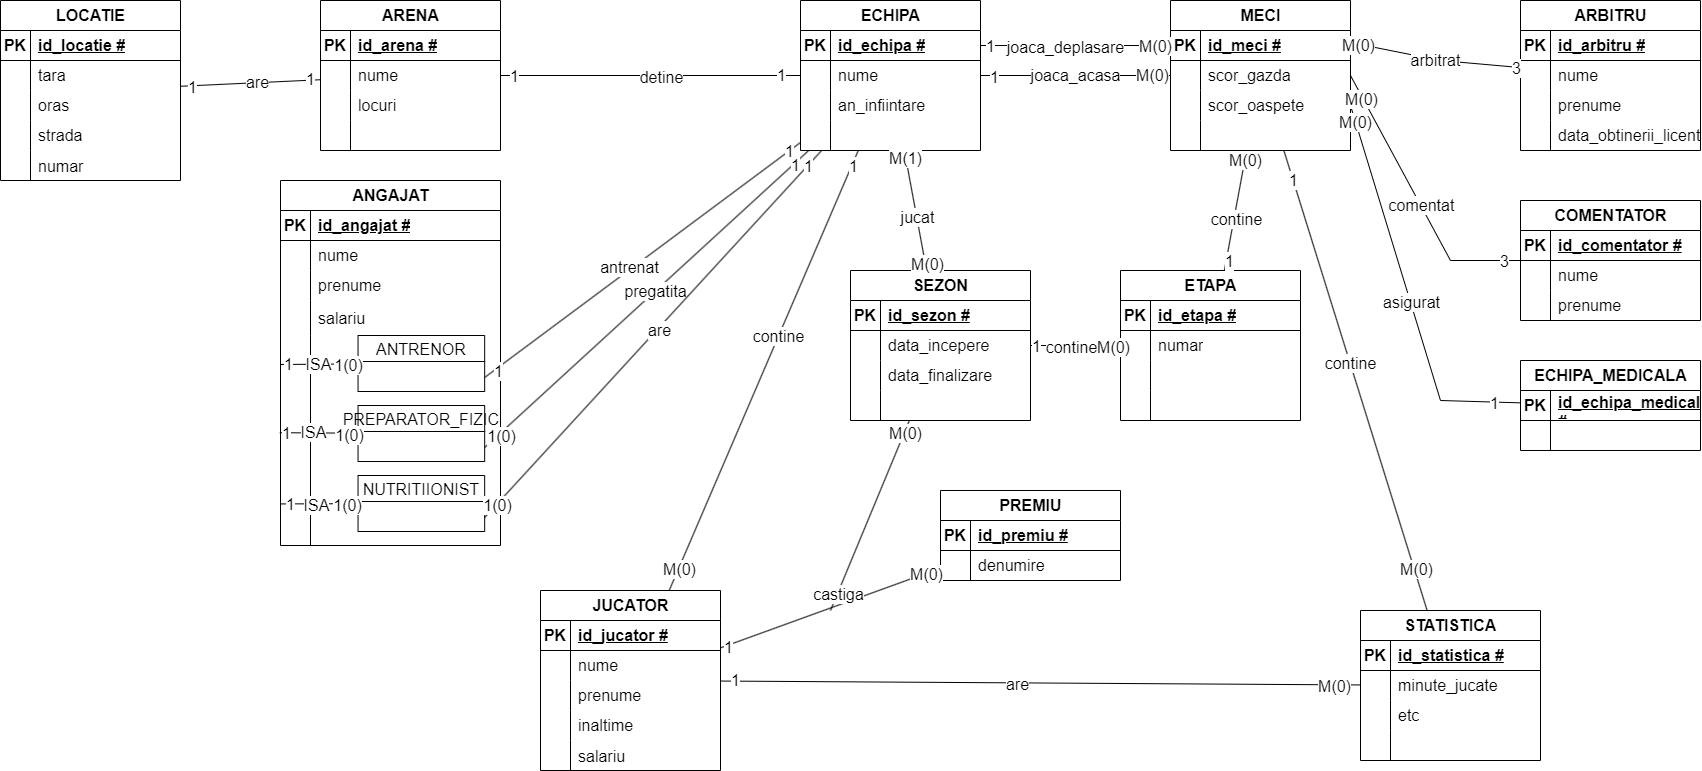
\includegraphics[width=\textwidth]{erd}
\end{center}
\pagebreak


\section{Diagrama Conceptuală}
Pornind de la diagrama entitate-relație realizați diagrama conceptuală a modelului propus, integrând
toate atributele necesare: entitățile, relațiile și atributele trebuie definite în limba română.

\begin{center}
	
	\vspace{1cm}
	
	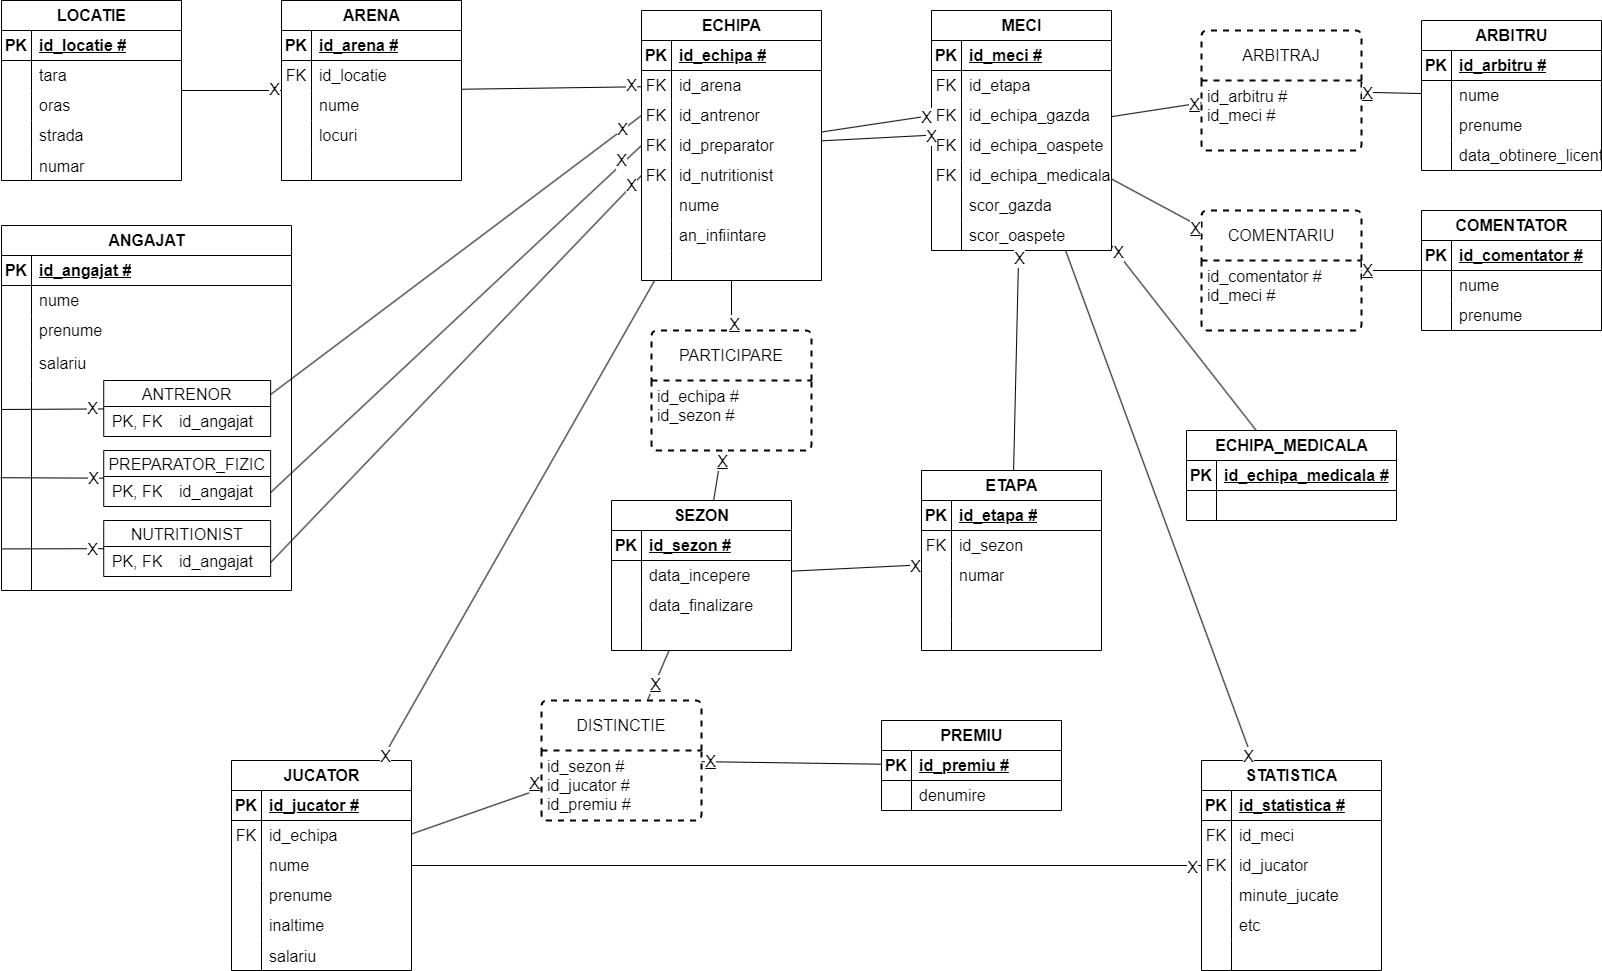
\includegraphics[width=\textwidth]{diagrama-conceptuala}
\end{center}
\pagebreak


\section{Implementarea Bazei de Date}
Implementați în Oracle diagrama conceptuală realizată: definiți toate tabelele, definind toate
constrângerile de integritate necesare (chei primare, cheile externe etc).

\subsection{Cod SQL}

\begin{multicols}{2}
\begin{lstlisting}
create sequence idseq
start with 1000
increment by 1
nocycle
nocache;

create table sezoane (
id_sezon number(7) primary key,
data_incepere date, 
data_finalizare date
);

create table etape(
id_etapa number(7) primary key, 
id_sezon number(7) references sezoane(id_sezon),
numar number(2)
);

create table angajati(
id_angajat number(7) primary key , 
nume varchar2(32),
prenume varchar2(32),
salariu number(7)
);

create table antrenori(
id_angajat number(7) primary key references angajati(id_angajat)
);

create table preparatori_fizici(
id_angajat number(7) primary key references angajati(id_angajat)
);

create table nutritionisti(
id_angajat number(7) primary key references angajati(id_angajat)
);

create table locatii (
id_locatie number(7) primary key, 
tara varchar2(32),
oras varchar2(32),
strada varchar2(32),
nr number(4)
);

create table arene (
id_arena number(7) primary key,
id_locatie number(7) references locatii(id_locatie),
nume varchar2(32),
locuri number(6)
);

create table echipe (
id_echipa number(7) primary key, 
id_arena number(7) references arene(id_arena),
id_antrenor number(7) references antrenori(id_angajat),
id_preparator number(7) references preparatori_fizici(id_angajat),
id_nutritionist number(7) references nutritionisti(id_angajat), 
nume varchar2(32), 
an_infiintare number(4)
);

create table jucatori(
id_jucator number(7) primary key, 
id_echipa number(7) references echipe(id_echipa),
nume varchar2(32),
prenume varchar2(32),
inaltime number(3, 2),
salariu number(7)
);

create table echipe_medicale(
id_echipa_medicala number(7) primary key
);

create table meciuri (
id_meci number(7) primary key,
id_etapa number(7) references etape(id_etapa),
id_echipa_gazda number(7) references echipe(id_echipa),
id_echipa_oaspete number(7) references echipe(id_echipa),
id_echipa_medicala number(7) references echipe_medicale(id_echipa_medicala),
scor_gazda number(3),
scor_oaspete number(3)
);

create table arbitrii(
id_arbitru number(7) primary key,
nume varchar2(32),
prenume varchar2(32),
data_obtinere_licenta date
);

create table comentatori (
id_comentator number(7) primary key,
nume varchar2(32),
prenume varchar2(32)
);

create table statistici(
id_statistica number(7) primary key,
id_meci number(7) references meciuri(id_meci),
id_jucator number(7) references jucatori(id_jucator),
minute_jucate number(2),
aruncari_2pct number(2),
aruncari_2pct_marcate number(2),
aruncari_3pct number(2),
aruncari_3pct_marcate number(2),
aruncari_libere number(2),
aruncari_libere_marcate number(2),
pase_decisive number(2),
recuperari number(2),
faulturi number(2)
);

create table premii(
id_premiu number(7) primary key,
denumire varchar2(64)
);

create table participari (
id_sezon number(7) references sezoane(id_sezon),
id_echipa number(7) references echipe(id_echipa),
constraint pk_participari primary key(id_sezon, id_echipa)
);

create table arbitraje(
id_meci number(7) references meciuri(id_meci),
id_arbitru number(7) references arbitrii(id_arbitru),
constraint pk_arbitraje primary key(id_meci, id_arbitru)
);

create table comentarii(
id_meci number(7) references meciuri(id_meci),
id_comentator number(7) references comentatori(id_comentator),
constraint pk_comentarii primary key(id_meci, id_comentator)
);

create table distinctii (
id_sezon number(7) references sezoane(id_sezon),
id_jucator number(7) references jucatori(id_jucator),
id_premiu number(7) references premii(id_premiu),
constraint pk_distinctii primary key(id_sezon, id_jucator, id_premiu)
);

savepoint after_create;
\end{lstlisting}
\end{multicols}

\pagebreak

\subsection {Capturi de Ecran}

\begin{multicols*}{4}

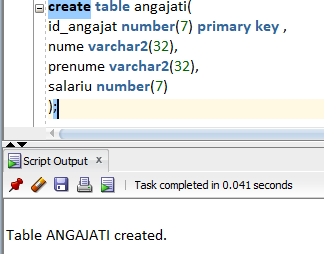
\includegraphics[width=\linewidth]{creation/angajati}
\vspace{4em}
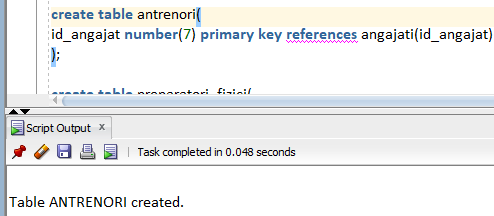
\includegraphics[width=\linewidth]{creation/antrenori}
\vspace{4em}
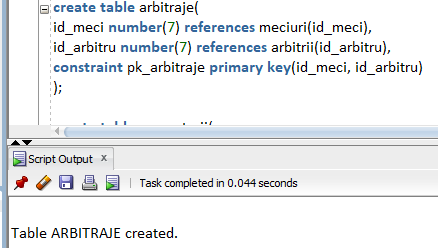
\includegraphics[width=\linewidth]{creation/arbitraje}
\vspace{4em}
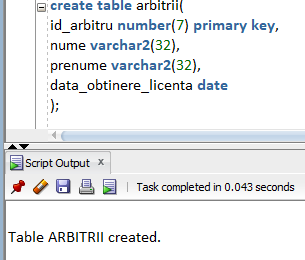
\includegraphics[width=\linewidth]{creation/arbitrii}
\vspace{4em}
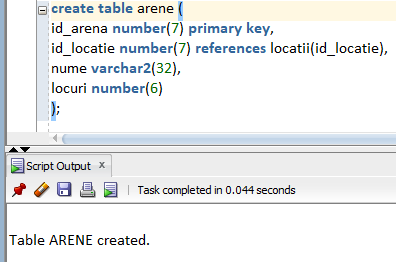
\includegraphics[width=\linewidth]{creation/arene}
\vspace{4em}
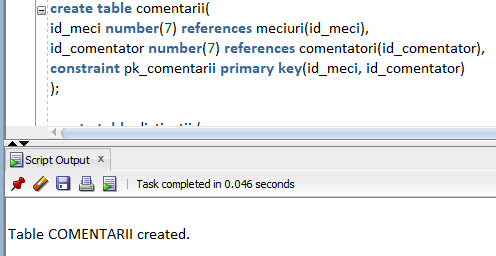
\includegraphics[width=\linewidth]{creation/comentarii}
\vspace{4em}
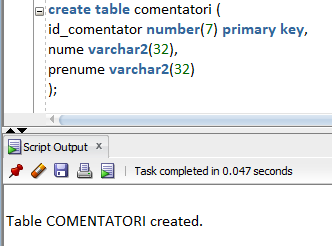
\includegraphics[width=\linewidth]{creation/comentatori}
\vspace{4em}
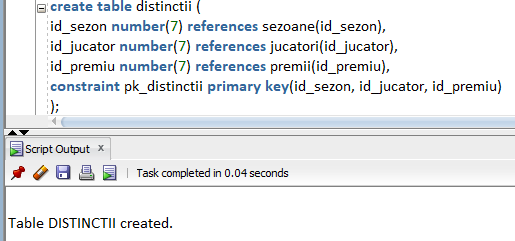
\includegraphics[width=\linewidth]{creation/distinctii}
\vspace{4em}
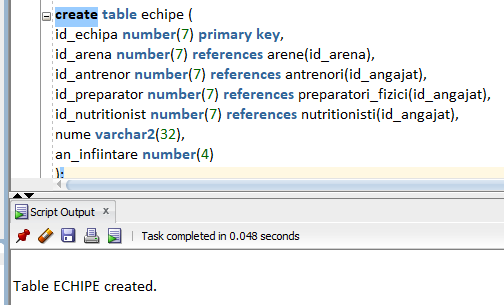
\includegraphics[width=\linewidth]{creation/echipe}
\vspace{4em}
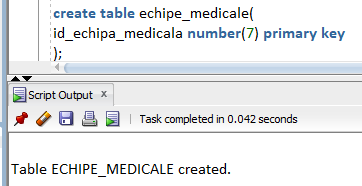
\includegraphics[width=\linewidth]{creation/echipe_medicale}
\vspace{4em}
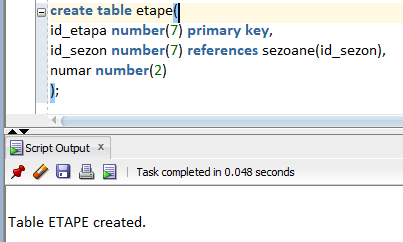
\includegraphics[width=\linewidth]{creation/etape}
\vspace{4em}
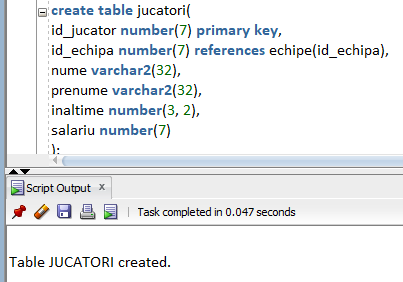
\includegraphics[width=\linewidth]{creation/jucatori}
\vspace{4em}
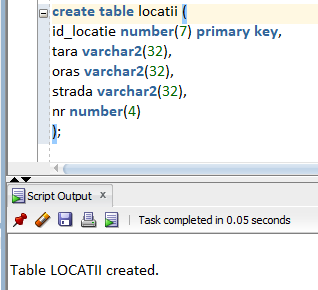
\includegraphics[width=\linewidth]{creation/locatii}
\vspace{4em}
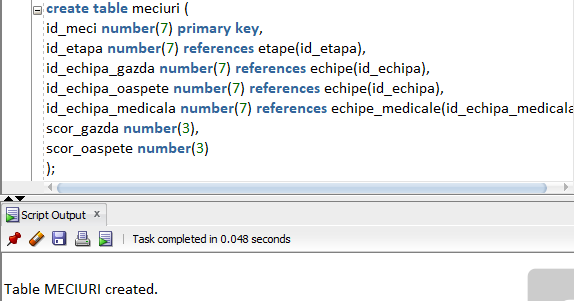
\includegraphics[width=\linewidth]{creation/meciuri}
\vspace{4em}
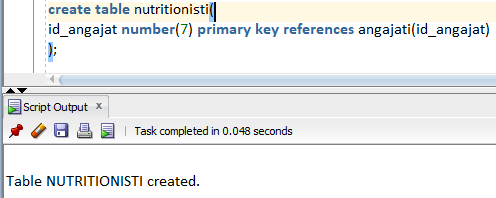
\includegraphics[width=\linewidth]{creation/nutritionisti}
\vspace{4em}
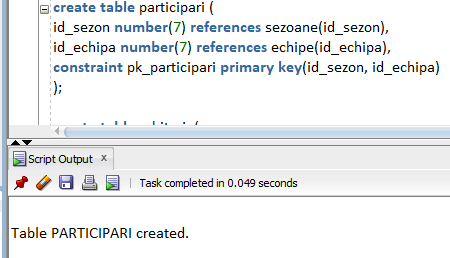
\includegraphics[width=\linewidth]{creation/participari}
\vspace{4em}
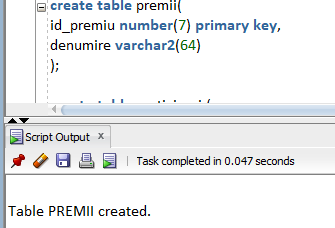
\includegraphics[width=\linewidth]{creation/premii}
\vspace{4em}
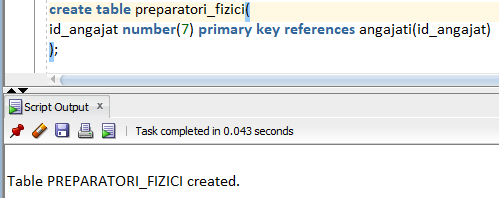
\includegraphics[width=\linewidth]{creation/preparatori}
\vspace{4em}
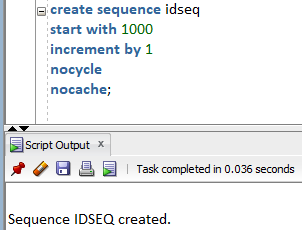
\includegraphics[width=\linewidth]{creation/sequence}
\vspace{4em}
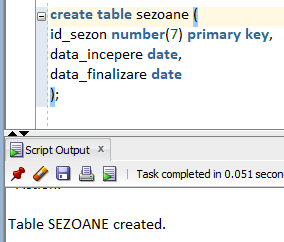
\includegraphics[width=\linewidth]{creation/sezoane}
\vspace{4em}
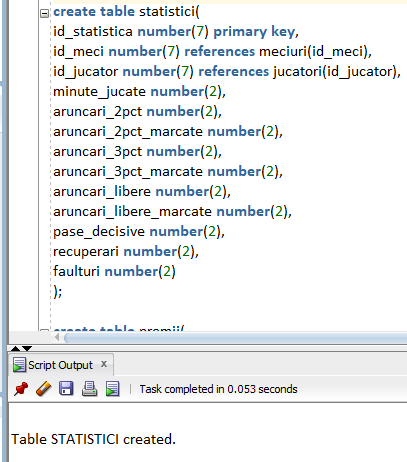
\includegraphics[width=\linewidth]{creation/statistici}
\vspace{4em}

\end{multicols*}


\section{Popularea Bazei de Date}
	Adăugați informații coerente în tabelele create (minim 5 înregistrări pentru fiecare entitate
	independentă; minim 10 înregistrări pentru tabela asociativă). 

\subsection{Cod Inserare}
Am ales să fac inserările utilizând PL/SQL din cauza numărului mare de informații stocate în baza de date. De asemenea, acest mod permite și modificarea datelor ce urmează a fi introduse, prin schimbări minore ale cod. În cazul în care utilizăm doar SQL, pentru fiecare cheie străină trebuia să știm valoarea să din tabela părinte dinainte, ceea ce limita cât de folositoare ar fi fost inserările scrise astfel.
\begin{multicols}{2}
\begin{lstlisting}
create or replace  function get_id    
return number is
f_id number;
begin
select idseq.nextval into f_id
from dual;
return f_id;
end;
/


create or replace function prenume_aleator
return varchar2 as 
prenume  varchar2(20);  
type StringArray is varray(20) of varchar2(20);
lista_prenume StringArray := StringArray(
'Ethan', 'Isaac', 'Leo', 'Miles', 'Asher',
'Maxwell', 'Oscar', 'Dylan', 'Oliver', 'Harrison',
'Nathan', 'Gabriel', 'Jasper', 'Ezra', 'Silas',
'Sebastian', 'Caleb', 'Gideon', 'Wyatt', 'Finn'
);
begin
prenume := lista_prenume(dbms_random.value(1, lista_prenume.last));
return prenume;
end;
/

create or replace function nume_aleator
return varchar2 as 
nume  varchar2(20);  
type StringArray is varray(50) of varchar2(20);
lista_nume StringArray := StringArray('Smith', 'Johnson', 'Williams', 'Jones', 'Brown', 
'Davis', 'Miller', 'Wilson', 'Moore', 'Taylor', 'Anderson', 'Thomas', 'Jackson',
'White', 'Harris', 'Martin', 'Thompson', 'Garcia', 'Martinez', 'Robinson', 'Clark', 
'Rodriguez', 'Lewis', 'Lee', 'Walker', 'Hall', 'Allen', 'Young', 'Hernandez', 'King', 
'Wright', 'Lopez', 'Hill', 'Scott', 'Green', 'Adams', 'Baker', 'Gonzalez', 'Nelson',
'Carter', 'Mitchell', 'Perez', 'Roberts', 'Turner', 'Phillips', 'Campbell', 'Parker', 'Evans', 'Edwards');


begin
nume := lista_nume(dbms_random.value(1, lista_nume.last));
return nume;
end;
/

begin
<<sterge_date>>
begin
delete from arbitraje;
delete from comentarii;
delete from distinctii;
delete from participari;


delete from premii;
delete from statistici;

delete from arbitrii;
delete from comentatori;
delete from meciuri;
delete from echipe_medicale;

delete from jucatori;
delete from echipe;
delete from arene;
delete from locatii;

delete from preparatori_fizici;
delete from nutritionisti;
delete from antrenori;
delete from angajati;

delete from etape;
delete from sezoane;
end;


<<insert_sezoane>>
declare
v_numar_sezoane number := 5;
v_format_data varchar2(11) := 'dd-mon-yyyy';
v_data_start date := to_date('15-aug-2022',v_format_data);
v_data_final date := to_date('10-jun-2023', v_format_data);
sezon sezoane%rowtype;
begin
sezon.data_incepere := v_data_start;
sezon.data_finalizare := v_data_final;
sezon.id_sezon := get_id();
for cnt in 1..v_numar_sezoane
loop
insert into sezoane
values sezon;
sezon.data_incepere := add_months(sezon.data_incepere, -12);
sezon.data_finalizare := add_months(sezon.data_finalizare, -12);
sezon.id_sezon := get_id();
end loop;

dbms_output.put_line('insert_sezoane OK');
end;

<<insert_etape>>
declare
v_numar_etape number := 30;
type id_sezoane is table of sezoane.id_sezon%type index by pls_integer;
v_id_sezoane id_sezoane; 
v_etapa etape%rowtype;
begin
select id_sezon
bulk collect into v_id_sezoane
from sezoane;

for cnt_sezon in v_id_sezoane.first..v_id_sezoane.last
loop
for cnt_etapa in 1..v_numar_etape
loop
v_etapa.id_etapa := get_id();
v_etapa.id_sezon := v_id_sezoane(cnt_sezon);
v_etapa.numar := cnt_etapa;
insert into etape
values v_etapa;
end loop;
end loop;
dbms_output.put_line('insert_etape OK');
end;

<<insert_antrenori>>
declare
numar_antrenori number := 16;
angajat angajati%rowtype;
antrenor antrenori%rowtype;
begin
for i in 1..numar_antrenori
loop
angajat.id_angajat := get_id();
angajat.nume := nume_aleator();
angajat.prenume := prenume_aleator();
angajat.salariu  := 100 * dbms_random.value(100, 200);
antrenor.id_angajat := angajat.id_angajat;

insert into angajati values angajat;
insert into antrenori values antrenor;
end loop;
dbms_output.put_line('insert_antrenori OK');
end;

<<insert_preparatori>>
declare
numar_preparatori number := 16;
angajat angajati%rowtype;
preparator preparatori_fizici%rowtype;
begin
for i in 1..numar_preparatori
loop
angajat.id_angajat := get_id();
angajat.nume := nume_aleator();
angajat.prenume := prenume_aleator();
angajat.salariu  := 100 * dbms_random.value(100, 200);
preparator.id_angajat := angajat.id_angajat;

insert into angajati values angajat;
insert into preparatori_fizici values preparator;
end loop;
dbms_output.put_line('insert_preparatori OK');
end;

<<insert_nutritionisti>>
declare
numar_nutritionisti number := 16;
angajat angajati%rowtype;
nutritionist nutritionisti%rowtype;
begin
for i in 1..numar_nutritionisti
loop
angajat.id_angajat := get_id();
angajat.nume := nume_aleator();
angajat.prenume := prenume_aleator();
angajat.salariu  := 100 * dbms_random.value(100, 200);
nutritionist.id_angajat := angajat.id_angajat;

insert into angajati values angajat;
insert into nutritionisti values nutritionist;
end loop;
dbms_output.put_line('insert_nutritionisti OK');
end;

<<insert_locatii>>
declare
type StringArray is varray(16) of varchar2(30);
orase StringArray := StringArray('New York City', 'Los Angeles','Las Vegas',
'Chicago', 'San Francisco', 'Miami', 'Orlando', 'Houston','Seattle', 
'Washington D.C.', 'Boston', 'Atlanta', 'Dallas', 'Denver',  
'New Orleans', 'San Diego');
strazi StringArray := StringArray('Fifth Avenue', 'Hollywood Boulevard', 
'Las Vegas Boulevard', 'Michigan Avenue', 'Lombard Street', 
'Ocean Drive', 'International Drive', 'NASA Road 1', 'Pike Place Market', 
'1600 Pennsylvania Avenue NW', 'Fenway Park',  'Peachtree Street', 
'Dealey Plaza', '16th Street Mall', 'Bourbon Street', 'Balboa Park');
locatie locatii%rowtype;
nr_locatii number := 16;
begin
for i in 1..nr_locatii
loop
locatie.id_locatie := get_id();
locatie.tara := 'USA';
locatie.oras := orase(i);
locatie.strada := strazi(i);
locatie.nr := dbms_random.value(100, 1000);
insert into locatii values locatie;
end loop;
dbms_output.put_line('insert_locatii OK');
end;

<<insert_arene>>
declare
type IdLocatii is table of locatii.id_locatie%type index by pls_integer;
id_locatii IdLocatii;
numar_arene number := 16;
type StringArray is varray(16) of varchar2(30);
lista_arene StringArray := StringArray('The Thunderdome', 'The Coliseum', 'The Pit', 
'The Garden',  'The Staples Center', 'The Oracle', 'The Hoop House', 'The Den',
'The Arena', 'The Thunderdome', 'The Dome', 'The Palace',
'The Madhouse', 'The Pavilion', 'The Buzzer Beater', 'The Swish Center');
arena arene%rowtype;
begin
select id_locatie
bulk collect into id_locatii
from locatii;

for i in 1..numar_arene
loop
arena.id_arena := get_id();
arena.id_locatie := id_locatii(i);
arena.nume := lista_arene(i);
arena.locuri := 1000 * dbms_random.value(10, 20);

insert into arene values arena;
end loop;
dbms_output.put_line('insert_arene OK');
end;

<<insert_echipe>>
declare
type StringArray is varray(16) of varchar2(20);
lista_nume StringArray := StringArray('Lightning Bolts', 'Thunderbirds', 
'Wildcats', 'Heatwave', 'Hurricanes', 'Jaguars', 'Patriots', 'Titans',
'Vikings', 'Dragons', 'Raptors', 'Warriors',
'Hornets', 'Sharks', 'Lions', 'Knights');

type IdTable is table of number index by pls_integer;
id_arene IdTable;
id_antrenori IdTable;
id_preparatori IdTable;
id_nutritionisti IdTable;
echipa echipe%rowtype;
numar_echipe number := 16;
begin
select id_arena bulk collect into id_arene from arene;
select id_angajat bulk collect into id_antrenori from antrenori;
select id_angajat bulk collect into id_preparatori from preparatori_fizici;
select id_angajat bulk collect into id_nutritionisti from nutritionisti;

for i in 1..numar_echipe
loop
echipa.id_echipa := get_id();
echipa.id_arena := id_arene(i);
echipa.id_antrenor := id_antrenori(i);
echipa.id_preparator := id_preparatori(i);
echipa.id_nutritionist := id_nutritionisti(i);
echipa.nume := lista_nume(i);
echipa.an_infiintare := 1960 + dbms_random.value(0, 30);

insert into echipe values echipa;
end loop;
dbms_output.put_line('insert_echipe OK');
end;    

<<insert_jucatori>>
declare
type IdArray is table of echipe.id_echipa%type index by pls_integer;
id_echipe IdArray;
id_echipa echipe.id_echipa%type;
jucator jucatori%rowtype;
numar_jucatori_per_echipa number := 5;
begin
select id_echipa bulk collect into id_echipe from echipe;

for i in id_echipe.first..id_echipe.last
loop
id_echipa := id_echipe(i);
for i in 1..numar_jucatori_per_echipa
loop
jucator.id_jucator := get_id();
jucator.id_echipa := id_echipa;
jucator.nume := nume_aleator();
jucator.prenume := prenume_aleator();
jucator.inaltime := dbms_random.value(1.80, 2.25);
jucator.salariu := 1000 * dbms_random.value(40, 100);

insert into jucatori values jucator;
end loop;
end loop;

dbms_output.put_line('insert_jucatori OK');
end;

<<insert_echipe_medicale>>
declare
numar_echipe_medicale number := 5;
begin
for i in 1..numar_echipe_medicale
loop 
insert into echipe_medicale values(get_id());
end loop;

dbms_output.put_line('insert_echipe_medicale OK');
end;

<<insert_meciuri>>
declare
type IdArray is table of number index by pls_integer;
id_sezoane IdArray;
id_echipe IdArray;
id_echipe_med IdArray;
id_etape IdArray;
meci meciuri%rowtype;
type IntArray is varray(8) of number;
x1 IntArray := IntArray(1, 2, 3, 4, 5, 6, 7, 8);
x2 IntArray := IntArray(16, 15, 14, 13, 12, 11, 10, 9);
rev boolean := false;
id_gazda number;
id_oaspete number;
temp number;
ids sezoane.id_sezon%type;
begin
select id_sezon bulk collect into id_sezoane from sezoane;
select id_echipa bulk collect into id_echipe from echipe;
select id_echipa_medicala bulk collect into id_echipe_med from echipe_medicale;



for i in id_sezoane.first..id_sezoane.last
loop
ids := id_sezoane(i);
select id_etapa bulk collect into id_etape 
from etape
where id_sezon = ids;

for nr_etapa in 1..30
loop
for i in 1..8
loop
if rev = false
then 
id_gazda := id_echipe(x1(i));
id_oaspete := id_echipe(x2(i));
else
id_gazda := id_echipe(x2(i));
id_oaspete := id_echipe(x1(i));
end if;

meci.id_meci := get_id();
meci.id_etapa := id_etape(nr_etapa);
meci.id_echipa_gazda := id_gazda;
meci.id_echipa_oaspete := id_oaspete;
meci.id_echipa_medicala := id_echipe_med(dbms_random.value(1, id_echipe_med.last));
meci.scor_gazda := dbms_random.value(60, 100);
meci.scor_oaspete := meci.scor_gazda + (dbms_random.value(0, 94) - 47);

insert into meciuri values meci;

end loop;
temp := x2(1);
for i in 1..7
loop
x2(i) := x2(i+1);
end loop;
x2(8) := x1(8);
for i in reverse 3..8
loop
x1(i) := x1(i-1);
end loop;
x1(2) := temp;

if x1(2) = 2
then rev := true;
end if;

end loop;
end loop;
end;    

<<insert_arbitrii>>
declare
arbitru arbitrii%rowtype;
numar_arbitrii number := 50;
begin
for i in 1..numar_arbitrii
loop
arbitru.nume := nume_aleator();
arbitru.prenume := prenume_aleator();
arbitru.id_arbitru := get_id();
arbitru.data_obtinere_licenta := to_date(trunc(
dbms_random.value(to_char(date '1990-01-01','J') ,to_char(date '2015-12-31','J') )
),'J' );
insert into arbitrii values arbitru;
end loop;

dbms_output.put_line('insert_arbitrii OK');
end;

<<insert_comentatori>>
declare
comentator comentatori%rowtype;
numar_comentatori number := 10;
begin
for i in 1..numar_comentatori
loop
comentator.nume := nume_aleator();
comentator.prenume := prenume_aleator();
comentator.id_comentator := get_id();
insert into comentatori values comentator;
end loop;

dbms_output.put_line('insert_comentatori OK');
end;


<<insert_statistici>>
declare
type IdArray is table of number index by pls_integer;
id_meciuri IdArray;
id_jucatori IdArray;
statistica statistici%rowtype;
meci meciuri%rowtype;
idm meciuri.id_meci%type;
idj jucatori.id_jucator%type;
begin
select id_meci bulk collect into id_meciuri from meciuri;

for i in id_meciuri.first..id_meciuri.last
loop
idm := id_meciuri(i);
select * into meci from meciuri where id_meci = idm;
select id_jucator bulk collect into id_jucatori
from jucatori
where id_echipa = meci.id_echipa_gazda or id_echipa = meci.id_echipa_oaspete;

for j in id_jucatori.first..id_jucatori.last
loop
idj := id_jucatori(j);
statistica.id_statistica := get_id();
statistica.id_meci := idm;
statistica.id_jucator := idj;
statistica.minute_jucate := dbms_random.value(20, 48);
statistica.aruncari_2pct := dbms_random.value(0, 30);
statistica.aruncari_2pct_marcate := dbms_random.value(0, statistica.aruncari_2pct);
statistica.aruncari_3pct := dbms_random.value(0, 20);
statistica.aruncari_3pct_marcate := dbms_random.value(0, statistica.aruncari_3pct);
statistica.aruncari_libere := dbms_random.value(0, 10);
statistica.aruncari_libere_marcate := dbms_random.value(0, statistica.aruncari_libere);
statistica.pase_decisive := dbms_random.value(0, 25);
statistica.recuperari := dbms_random.value(0,15);
statistica.faulturi := dbms_random.value(0, 5);

insert into statistici values statistica;
end loop;
end loop;

dbms_output.put_line('insert_statistica OK');
end;

<<insert_premii>>
declare
type StringArray is varray(5) of varchar2(50);
lista_premii StringArray := StringArray('Most Valuable Player (MVP)', 
'Team Player of the Year',
'Defensive Player of the Year', 'Sportsmanship Award', 'Best Distance Shooter');
premiu premii%rowtype;
begin
for i in lista_premii.first..lista_premii.last
loop
premiu.id_premiu := get_id();
premiu.denumire := lista_premii(i);
insert into premii values premiu;
end loop;

dbms_output.put_line('inser_premii OK');
end;

<<insert_participari>>
declare
type IdArray is table of number index by pls_integer;
id_sezoane IdArray;
id_echipe IdArray;
participare participari%rowtype;
ids sezoane.id_sezon%type;
ide echipe.id_echipa%type;
begin
select id_sezon bulk collect into id_sezoane from sezoane;
select id_echipa bulk collect into id_echipe from echipe;

for i in id_sezoane.first..id_sezoane.last
loop
ids := id_sezoane(i);
for j in id_echipe.first..id_echipe.last
loop
ide := id_echipe(j);
participare.id_sezon := ids;
participare.id_echipa := ide;
insert into participari values participare;
end loop;
end loop;

dbms_output.put_line('insert_participari OK');
end;

<<insert_comentarii>>
declare
comentariu comentarii%rowtype;
type IdArray is table of number index by pls_integer;
id_meciuri IdArray;
id_comentatori IdArray;
a number(2,0);
b number(2,0);
c number(2,0);
begin
select id_meci bulk collect into id_meciuri from meciuri;
select id_comentator bulk collect into id_comentatori from comentatori;

for i in id_meciuri.first..id_meciuri.last
loop
a := dbms_random.value(1,id_comentatori.last);
b := dbms_random.value(1,id_comentatori.last);
c := dbms_random.value(1,id_comentatori.last);
while a = b
loop
b := dbms_random.value(1,id_comentatori.last);
end loop;
while a = c or b = c
loop
c := dbms_random.value(1,id_comentatori.last);
end loop;
comentariu.id_meci := id_meciuri(i);
comentariu.id_comentator := id_comentatori(a);
insert into comentarii values comentariu;
comentariu.id_comentator := id_comentatori(b);
insert into comentarii values comentariu;
comentariu.id_comentator := id_comentatori(c);
insert into comentarii values comentariu;
end loop;

dbms_output.put_line('insert-comentarii OK');
end;

<<insert_arbitraje>>
declare
arbitraj arbitraje%rowtype;
type IdArray is table of number index by pls_integer;
id_meciuri IdArray;
id_arbitrii IdArray;
a number(2,0);
b number(2,0);
c number(2,0);
begin
select id_meci bulk collect into id_meciuri from meciuri;
select id_arbitru bulk collect into id_arbitrii from arbitrii;

for i in id_meciuri.first..id_meciuri.last
loop
a := dbms_random.value(1,id_arbitrii.last);
b := dbms_random.value(1,id_arbitrii.last);
c := dbms_random.value(1,id_arbitrii.last);
while a = b
loop
b := dbms_random.value(1,id_arbitrii.last);
end loop;
while a = c or b = c
loop
c := dbms_random.value(1,id_arbitrii.last);
end loop;
arbitraj.id_meci := id_meciuri(i);
arbitraj.id_arbitru := id_arbitrii(a);
insert into arbitraje values arbitraj;
arbitraj.id_arbitru := id_arbitrii(b);
insert into arbitraje values arbitraj;
arbitraj.id_arbitru := id_arbitrii(c);
insert into arbitraje values arbitraj;
end loop;

dbms_output.put_line('insert-arbitraje OK');
end;

<<insert_distinctii>>
declare
distinctie distinctii%rowtype;
type IdArray is table of number index by pls_integer;
id_sezoane IdArray;
id_jucatori IdArray;
id_premii IdArray;
begin
select id_sezon bulk collect into id_sezoane from sezoane;
select id_jucator bulk collect into id_jucatori from jucatori;
select id_premiu bulk collect into id_premii from premii;

for i in id_sezoane.first..id_sezoane.last
loop
for j in id_premii.first..id_premii.last
loop
distinctie.id_sezon := id_sezoane(i);
distinctie.id_premiu := id_premii(j);
distinctie.id_jucator := id_jucatori(dbms_random.value(1, id_jucatori.last));

insert into distinctii values distinctie;
end loop;
end loop;

dbms_output.put_line('insert_distinctii OK');
end;

<<verifica_inserare>>
declare
cnt number;
type StringArray is varray(20) of varchar2(20);
tabele StringArray := StringArray('angajati', 'antrenori', 'arbitrii', 
'arene', 'comentarii', 'comentatori', 'distinctii', 'echipe', 
'echipe_medicale', 'etape', 'jucatori', 'locatii', 
'meciuri', 'nutritionisti', 'participari', 'premii', 'preparatori_fizici', 
'sezoane', 'statistici');
begin
select count(*) into cnt from angajati;
dbms_output.put_line('Exista ' || cnt || ' angajati.');
select count(*) into cnt from antrenori;
dbms_output.put_line('Exista ' || cnt || ' antrenori.');   
select count(*) into cnt from arbitraje;
dbms_output.put_line('Exista ' || cnt || ' arbitraje.');
select count(*) into cnt from arbitrii;
dbms_output.put_line('Exista ' || cnt || ' arbitrii.');
select count(*) into cnt from arene;
dbms_output.put_line('Exista ' || cnt || ' arene.');
select count(*) into cnt from comentarii;
dbms_output.put_line('Exista ' || cnt || ' comentarii.');   
select count(*) into cnt from comentatori;
dbms_output.put_line('Exista ' || cnt || ' comentatori.');   
select count(*) into cnt from distinctii;
dbms_output.put_line('Exista ' || cnt || ' distinctii.');
select count(*) into cnt from echipe;
dbms_output.put_line('Exista ' || cnt || ' echipe.');
select count(*) into cnt from echipe_medicale;
dbms_output.put_line('Exista ' || cnt || ' echipe_medicale.');
select count(*) into cnt from etape;
dbms_output.put_line('Exista ' || cnt || ' etape.');   
select count(*) into cnt from jucatori;
dbms_output.put_line('Exista ' || cnt || ' jucatori.');
select count(*) into cnt from locatii;
dbms_output.put_line('Exista ' || cnt || ' locatii.');
select count(*) into cnt from meciuri;
dbms_output.put_line('Exista ' || cnt || ' meciuri.');
select count(*) into cnt from nutritionisti;
dbms_output.put_line('Exista ' || cnt || ' nutritionisti.');   
select count(*) into cnt from participari;
dbms_output.put_line('Exista ' || cnt || ' participari.');
select count(*) into cnt from premii;
dbms_output.put_line('Exista ' || cnt || ' premii.');
select count(*) into cnt from preparatori_fizici;
dbms_output.put_line('Exista ' || cnt || ' preparatori_fizici.');   
select count(*) into cnt from sezoane;
dbms_output.put_line('Exista ' || cnt || ' sezoane.');
select count(*) into cnt from statistici;
dbms_output.put_line('Exista ' || cnt || ' statistici.');

end;
dbms_output.put_line('OK');
end;
/



\end{lstlisting}
\end{multicols}
\subsection{Captură de Ecran}
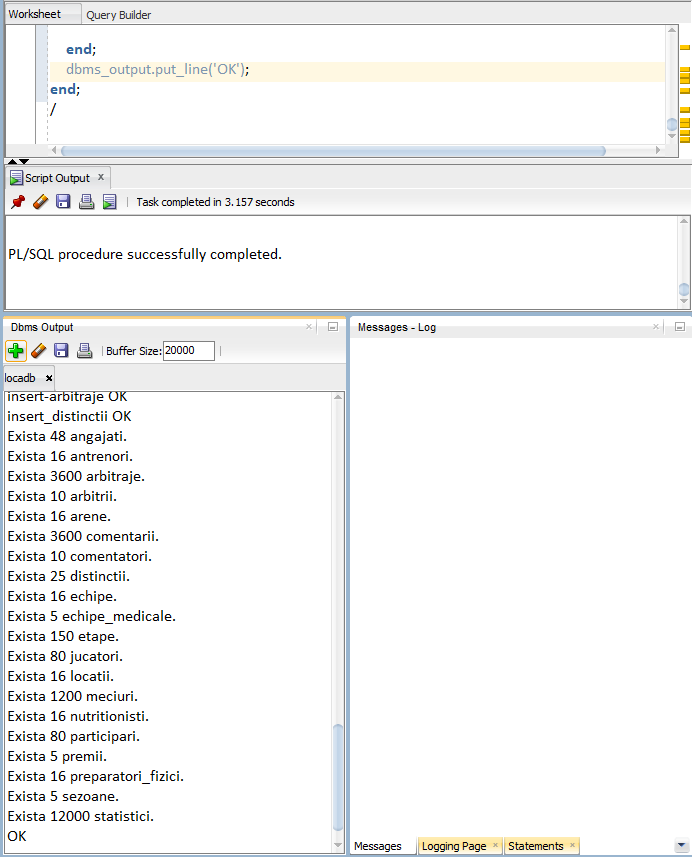
\includegraphics[width=36em,keepaspectratio]{insert}
\pagebreak


\section{Problema - Colecții de Date}
	Formulați în limbaj natural o problemă pe care să o rezolvați folosind un subprogram stocat
	independent care să utilizeze toate cele 3 tipuri de colecții studiate. Apelați subprogramul.
	
\subsection{Cerință}
În fiecare etapă se determina clasamentul celor mai buni 3 jucători (cu cele mai multe puncte în meciul din etapă respectivă) din echipele care au ieșit câștigătoare, primind titlul de "Jucătorii Etapei". După aceea, pentru fiecare sezon, se cumulează punctele fiecărui "Jucător al Etapei" (doar din etapele în care a primit acest titlu) și se realizează clasamentul final. Jucătorul cu cele mai multe puncte primește premiul "MVP (most valuable player)".
Pentru fiecare sezon, să se afișeze numele, prenumele și salariul jucătorului care a primit această distincție, precum și numărul de puncte cumulate.

\subsection{Rezolvare}
\begin{lstlisting}
-- ex 6
create or replace procedure ex6_colectii 
as
-- Am ales tabloul imbricat deoarece numarul de sezoane este necunoscut 
-- si nu fac stergeri pe parcursul programului
type IdSezoane is table of sezoane.id_sezon%type ;
id_sezoane IdSezoane;
id_sezon_curent sezoane.id_sezon%type;

-- Am ales varray deoarece stiu dinainte numarul de etape (30) dintr-un sezon,
-- respectiv numarul de meciuri dintr-o etapa (8), si nu fac stergeri in aceasta colectie
type IdEtape is varray(30) of etape.id_etapa%type;
id_etape IdEtape;
id_etapa_curenta sezoane.id_sezon%type;

type RecordJucator is record
(
id_jucator jucatori.id_jucator%type,
puncte number
);
type idJucatoriTop3 is varray(3) of RecordJucator;
id_jucatori_3 IdJucatoriTop3;
rec RecordJucator;

-- Am ales tablou indexat deoarece indicii vor fi anumite id-uri ale jucatorilor, nu neaparat dense.
type TabelPuncteJucatori is table of number(4) index by pls_integer;
puncte_jucator TabelPuncteJucatori := TabelPuncteJucatori();

nr_etape number; -- restriciile spun ca pentru fiecare sezon exista 30 etape

maxim number;
id_mvp jucatori.id_jucator%type;
jucator jucatori%rowtype;

begin
select id_sezon bulk collect into id_sezoane from sezoane;

for it_sezon in id_sezoane.first..id_sezoane.last loop
id_sezon_curent := id_sezoane(it_sezon);
select count(id_etapa) collect into nr_etape 
from etape
where id_sezon = id_sezon_curent;

if nr_etape != 30
then 
dbms_output.put_line ('In sezonul ' || id_sezon_curent || 
' nu sunt 30 de etape ( ' || nr_etape || ' )');
continue;
end if;

select id_etapa bulk collect into id_etape 
from etape
where id_sezon = id_sezon_curent;

puncte_jucator := TabelPuncteJucatori();
maxim := 0;
for it_etapa in id_etape.first..id_etape.last loop
id_etapa_curenta := id_etape(it_etapa);
with jucatori_si_puncte as
(select j.id_jucator, 2 * aruncari_2pct_marcate + 3 * aruncari_3pct_marcate + aruncari_libere_marcate
from jucatori j
join meciuri m on m.id_etapa = id_etapa_curenta and
((m.id_echipa_gazda = j.id_echipa and scor_gazda >  scor_oaspete ) or
(m.id_echipa_oaspete = j.id_echipa and scor_gazda <  scor_oaspete ))
join statistici s on s.id_meci = m.id_meci and s.id_jucator = j.id_jucator
order by 2 desc)
select * bulk collect into id_jucatori_3
from jucatori_si_puncte
where rownum <= 3;

for it in id_jucatori_3.first..id_jucatori_3.last loop
rec := id_jucatori_3(it);
if puncte_jucator.exists(rec.id_jucator) = false
then puncte_jucator(rec.id_jucator) := 0;
end if;

puncte_jucator(rec.id_jucator) := puncte_jucator(rec.id_jucator) + rec.puncte;
if maxim < puncte_jucator(rec.id_jucator)
then
maxim := puncte_jucator(rec.id_jucator);
id_mvp := rec.id_jucator;
end if;
end loop;
end loop;

select * into jucator
from jucatori
where id_jucator = id_mvp;

dbms_output.put_line(jucator.nume || ' ' || jucator.prenume || '  id: ' || id_mvp || ' puncte:  ' || puncte_jucator(id_mvp));

end loop;

end;
/

begin
ex6_colectii();
end;
/



\end{lstlisting}

\subsection {Captură de Ecran}
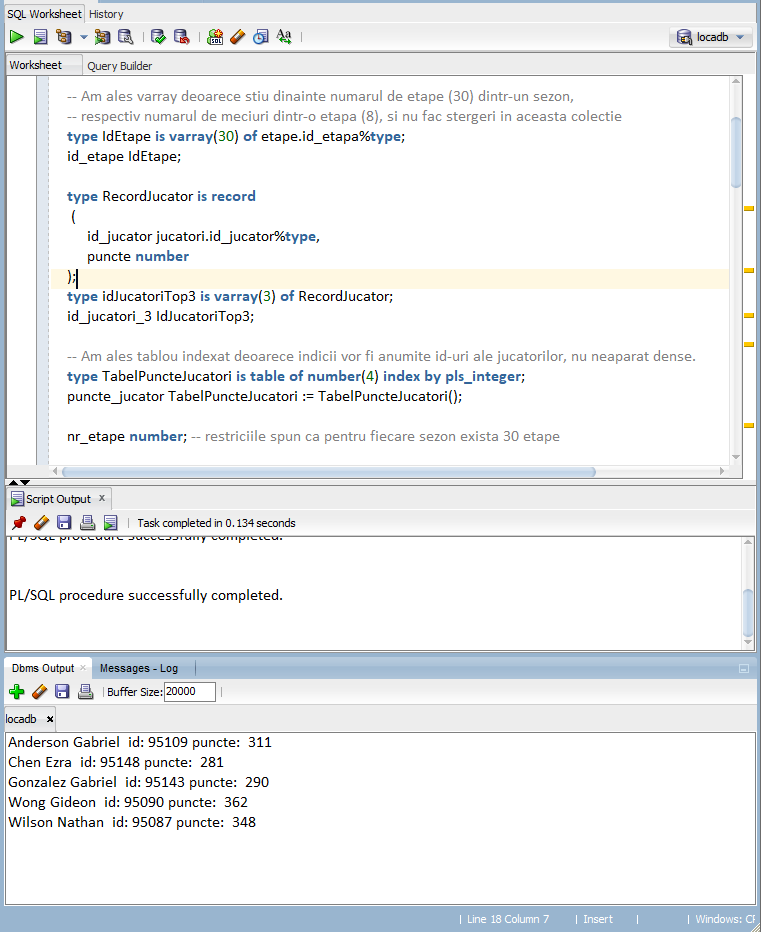
\includegraphics[width=32em,keepaspectratio]{rez_colectii}
\pagebreak

\section{Problemă - Cursoare}
	Formulați în limbaj natural o problemă pe care să o rezolvați folosind un subprogram stocat
	independent care să utilizeze 2 tipuri diferite de cursoare studiate, unul dintre acestea fiind cursor
	parametrizat, dependent de celălalt cursor. Apelați subprogramul.
	
\subsection{Cerință}
Se bănuiește că există arbitrii care au influențat rezultatele meciurilor. 
Comisia a hotărât să găsească meciurile în care diferența de puncte este maximă și să verifice dacă arbitrajul a fost realizat de arbitrii care au legătură cu vreun jucător de pe teren (au același nume de familie).
Să se găsească toate aceste perechi, afișându-se, pentru fiecare:
\begin{verbatim}
	IdMeci: NumeArbitru PrenumeArbitru - NumeJucator PrenumeJucator - ScorMeci - Mesaj
\end{verbatim}
Mesajul ne spune daca jucătorul care are legătură cu arbitrul s-a aflat in echipa câștigătoare sau cea înfrântă.

\subsection{Rezolvare}
\begin{lstlisting}
create or replace procedure ex7_cursoare
is
cursor c_id_arbitri (idm meciuri.id_meci%type) is
select id_arbitru from arbitraje where arbitraje.id_meci = idm;


type IdArbitri is table of arbitrii.id_arbitru%type;
id_arbitri IdArbitri;
arbitru arbitrii%rowtype;

cursor meciuriVerificate is
select *
from meciuri
where abs(scor_gazda - scor_oaspete) =  
(select max(abs(scor_gazda - scor_oaspete))
from meciuri);

cursor arbitriVerificati (idm meciuri.id_meci%type) is
select *
from arbitrii
where id_arbitru in (select id_arbitru from arbitraje where arbitraje.id_meci = idm);

cursor jucatoriMeci (
id_gazda echipe.id_echipa%type,
id_oaspete echipe.id_echipa%type, 
nume_arbitru arbitrii.nume%type) is
select id_jucator , nume, prenume, id_echipa
from jucatori 
where (id_echipa = id_gazda or id_echipa = id_oaspete)
and jucatori.nume = nume_arbitru;

mesaj varchar2(50);
id_echipa echipe.id_Echipa%type;
begin

-- CICLU CURSOR
for meci in meciuriVerificate loop
--        dbms_output.put_line('meci: ' || meci.id_meci);

-- CURSOR CLASIC PARAMETRIZAT
open c_id_arbitri(meci.id_meci);
fetch c_id_arbitri bulk collect into id_arbitri;
close c_id_arbitri;

for i in id_arbitri.first..id_arbitri.last loop
select * into arbitru
from arbitrii
where id_arbitru = id_arbitri(i);
--            dbms_output.put_line('arbitru: ' || arbitru.id_arbitru);
-- CICLU CURSOR PARAMETRIZAT
for jucator in jucatoriMeci(meci.id_echipa_gazda, meci.id_echipa_oaspete, arbitru.nume) loop

if meci.scor_gazda > meci.scor_oaspete
then id_echipa := meci.id_echipa_gazda;
else id_echipa := meci.id_echipa_oaspete;
end if;

if jucator.id_echipa = id_echipa
then mesaj := ' (Victorie)';
else mesaj := ' (Infrangere)';
end if;

dbms_output.put_line(meci.id_meci || ': ' ||
arbitru.id_arbitru || ' ' || arbitru.nume || ' ' || arbitru.prenume || ' - ' ||
jucator.id_jucator || ' ' || jucator.nume || ' ' || jucator.prenume || ' - ' || 
meci.scor_gazda || '-' || meci.scor_oaspete || mesaj);

end loop;
end loop;
end loop;

end;
/

begin
ex7_cursoare();
end;
/


\end{lstlisting}

\subsection{Captura de Ecran}
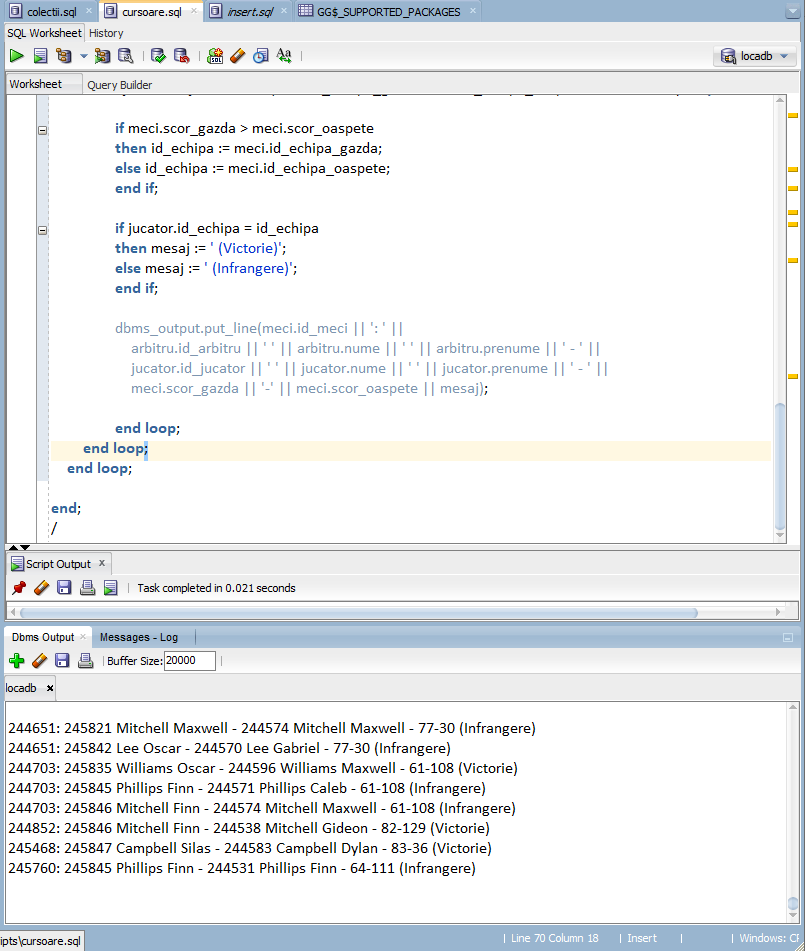
\includegraphics[width=30em, keepaspectratio]{cursoare}
\pagebreak
\section{Problema - Excepții}
	Formulați în limbaj natural o problemă pe care să o rezolvați folosind un subprogram stocat
	independent de tip funcție care să utilizeze într-o singură comandă SQL 3 dintre tabelele definite.
	Definiți minim 2 excepții proprii. Apelați subprogramul astfel încât să evidențiați toate cazurile
	definite și tratate
\subsection{Cerință}
Se da un prenume P și un salariu minim S. Pentru fiecare echipa se calculează suma salariilor jucătorilor și angajaților cu prenumele P și salariul mai mare sau egal decât S. Să se afișeze numele echipelor care au cel puț în un angajat sau jucător care respectă condițiile și suma calculată , în ordine descrescătoare a sumei. Funcția va retuna suma tuturor salariilor ce respectă condițiile . Să se trateze cazurile în care nu există niciun jucător sau angajat cu prenumele P, respectiv cazul în care niciun jucător sau angajat cu prenumele P nu are salariul mai mare sau egal decât S.

\subsection{Rezolvare}
\begin{lstlisting}
create or replace function ex8_exceptii
(p_prenume in varchar2,
p_salariu_minim in number)
return number
is
ex_no_first_name exception;
ex_no_salary exception;
type RecordEchipa is Record (
--        id_echipa echipe.id_echipa%type,
nume varchar2(50),
suma_salarii number
);
type ListaEchipe is table of RecordEchipa;
lista_echipe ListaEchipe;

aux number := 0;

begin
select count(*) collect into aux
from (select id_jucator from jucatori where lower(prenume) like lower(p_prenume)
union select id_angajat from angajati where lower(prenume) like lower(p_prenume));

if aux = 0 then
raise ex_no_first_name;
end if;

with persoane as (
select e.id_echipa id_echipa, salariu 
from angajati a
join echipe e on e.id_antrenor = a.id_angajat or e.id_preparator = a.id_angajat 
or e.id_nutritionist = a.id_angajat
where lower(a.prenume) like lower(p_prenume) and a.salariu >= p_salariu_minim
union
select id_echipa, salariu from jucatori
where lower(prenume) like lower(p_prenume) and salariu >= p_salariu_minim
)
select * bulk collect into lista_echipe
from (
select e.nume, sum(p.salariu) 
from persoane p
join echipe e on e.id_echipa = p.id_echipa
group by e.nume
)
order by 2 desc;


if lista_echipe.count = 0 then
raise ex_no_salary;
end if;

aux := 0;
for i in lista_Echipe.first..lista_echipe.last loop
dbms_output.put_line(lista_echipe(i).nume || ' - ' || lista_echipe(i).suma_salarii);
aux := aux + lista_echipe(i).suma_salarii;
end loop;

return aux;

exception
when ex_no_first_name then
dbms_output.put_line('Exceptie: nu exista prenumele ' || p_prenume);
return 0;
when ex_no_salary then
dbms_output.put_line('Exceptie: nu exista salarii mai mari decat ' || p_salariu_minim);
return 0;
when others then
dbms_output.put_line('Alta Exceptie');
return 0;
end;
/

begin

dbms_output.put_line(ex8_exceptii('isaac', 50000));
dbms_output.put_line(ex8_exceptii('prenume', 1000));
dbms_output.put_line(ex8_exceptii('isaac', 100000));
end;
/
\end{lstlisting}

\subsection{Captură de Ecran}
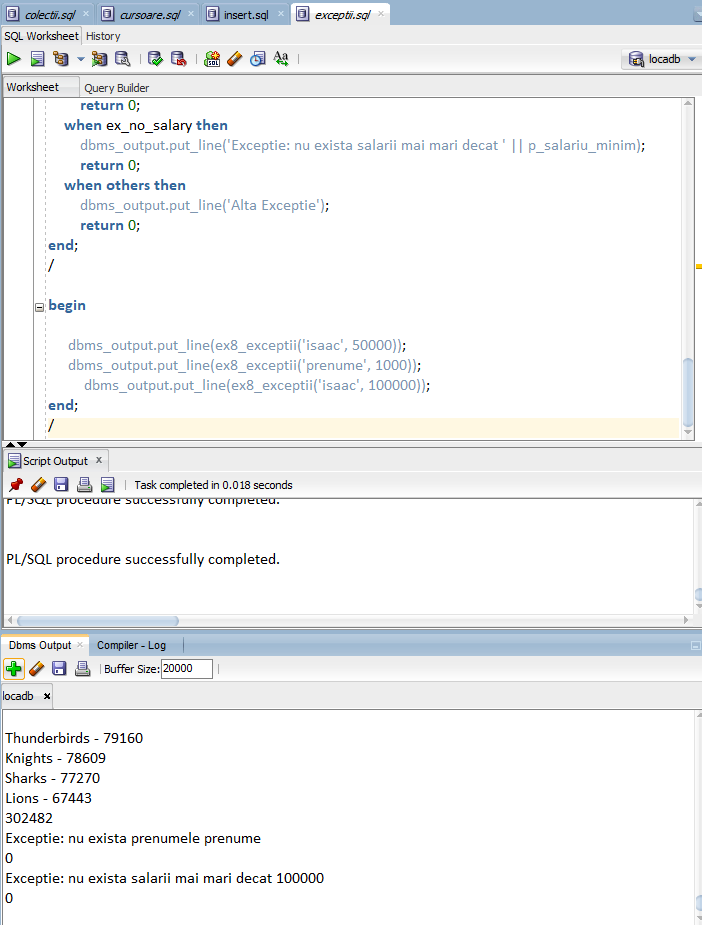
\includegraphics[width=30em, keepaspectratio]{rez_exceptii8}
\pagebreak

\section{Problemă - Subprogram de Tip Procedura}
	Formulați în limbaj natural o problemă pe care să o rezolvați folosind un subprogram stocat
	independent de tip procedură care să utilizeze într-o singură comandă SQL 5 dintre tabelele
	definite. Tratați toate excepțiile care pot apărea, incluzând excepțiile NO\_DATA\_FOUND și
	TOO\_MANY\_ROWS. Apelați subprogramul astfel încât să evidențiați toate cazurile tratate.

\subsection{Cerință}
Se știe numele unui angajat. Să se afișeze numele echipei pentru care lucrează și postul acestuia. Pentru echipa în care acesta lucrează ( să se afișeze numele și id-ul), să se afle jucătorii care au câștigat primit cel puț în o distincție . Pentru fiecare dintre aceștia să se afișeze următoarele statistici: procentajul aruncărilor de 3 puncte marcate, procentajul meciurilor in care a faultat și numărul mediu de pase decisive.
\subsection{Rezolvare}
\begin{lstlisting}
create or replace procedure exceptii_ex9
(p_nume in angajati.nume%type
)
is
ex_no_player exception;
type RecAngajat is record (
nume angajati.nume%type, 
prenume angajati.prenume%type,
nume_echipa echipe.nume%type, 
post varchar2(20)
);
angajat RecAngajat;
type RecEchipa is record (
id echipe.id_echipa%type,
nume echipe.nume%type);
echipa RecEchipa;

type RecJucator is record(
id jucatori.id_jucator%type,
nume jucatori.nume%type, 
prenume jucatori.prenume%type, 
proc_3pct number(5, 2), 
proc_faulturi number(5, 2),
avg_pase number(5, 2)
);
type ListaJucatori is table of RecJucator;
lista_jucatori ListaJucatori;

begin

select a.nume, a.prenume, e.nume, (case
when a.id_angajat = e.id_antrenor then 'antrenor'
when a.id_angajat = e.id_preparator then 'preparator fizic'
when a.id_angajat = e.id_nutritionist then 'nutritionist'
end) post
into angajat
from angajati a, echipe e
where lower(a.nume) = lower(p_nume)
and id_angajat in (e.id_antrenor, e.id_preparator, e.id_nutritionist);

dbms_output.put_line(angajat.nume || ' ' || angajat.prenume || ' lucreaza pentru echipa ' || 
angajat.nume_echipa || ' pe postul de ' || angajat.post);

with info_echipa as (
select id_echipa, e.nume
from echipe e 
where (p_nume) in
(select nume
from angajati
where lower(nume) = lower(p_nume)
and id_angajat in (e.id_antrenor, e.id_preparator, e.id_nutritionist))
)
select j.id_jucator, j.nume, j.prenume, 100 * sum(s.aruncari_3pct_marcate) / sum(s.aruncari_3pct),
100 * sum(case when s.faulturi > 0 then 1 else 0 end) / count(*), avg(s.pase_decisive)
bulk collect into lista_jucatori
from jucatori j
join statistici s on s.id_jucator = j.id_jucator
where j.id_jucator in (select distinct id_jucator from distinctii)
and j.id_echipa = (select id_echipa from info_echipa)
group by (j.id_jucator, j.nume, j.prenume);

if lista_jucatori.count = 0 then
raise ex_no_player;
end if;

for i in lista_jucatori.first..lista_jucatori.last loop
dbms_output.put_line(lista_jucatori(i).nume || ' ' || lista_jucatori(i).prenume || ' -  procentaj 3pct: ' 
|| lista_jucatori(i).proc_3pct || '% - procentaj meciuri cu fault:  ' || lista_jucatori(i).proc_faulturi || 
'% - medie pase decisive: ' || lista_jucatori(i).avg_pase);
end loop;

exception
when no_data_found then
dbms_output.put_line('Nu exista niciun angajat cu numele ' || p_nume);
when too_many_rows then
dbms_output.put_line('Exista mai multi angajati cu numele ' || p_nume);
when ex_no_player then
dbms_output.put_line('Nu exista niciun jucator care sa fi primit vreo distinctie in echipa ' || angajat.nume_echipa);
end;
/

begin
dbms_output.put_line('Apel cu numele: Johnson');
exceptii_ex9('Johnson');
dbms_output.put_line('Apel cu numele: Carter');
exceptii_ex9('Carter');
dbms_output.put_line('Apel cu numele: Clark');
exceptii_ex9('Clark');
dbms_output.put_line('Apel cu numele: John');
exceptii_ex9('John');
end;

/
\end{lstlisting}

\subsection{Captură de Ecran}
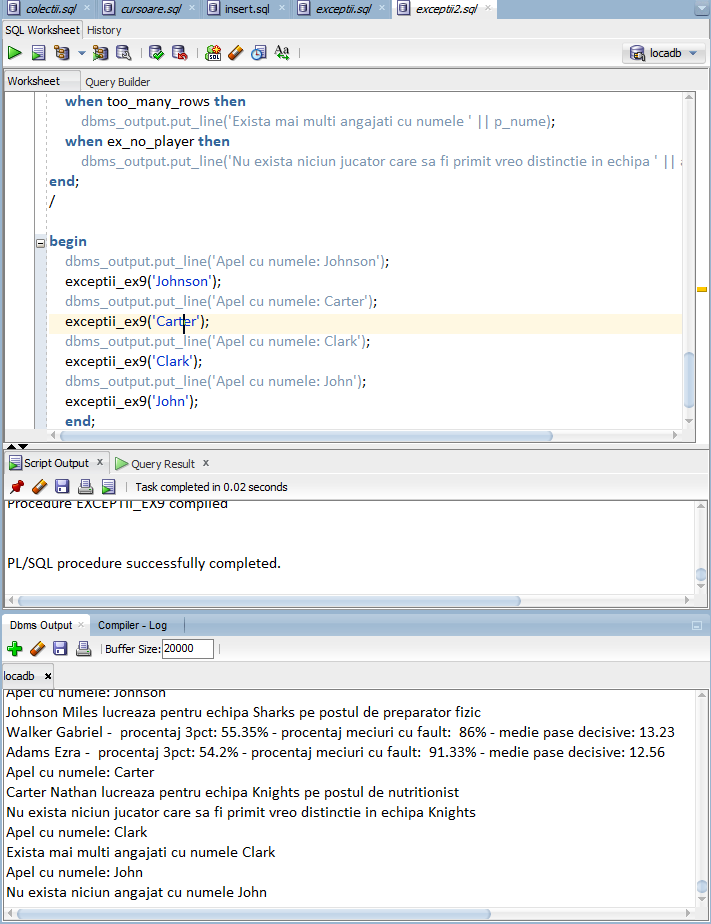
\includegraphics[width=40em, keepaspectratio]{rez_exceptii9}
\pagebreak
\section{Problemă - Trigger LMD la nivel de comanda}
	Definiți un trigger de tip LMD la nivel de comandă. Declanșați trigger-ul.
	
\subsection{Cerință}
Să se definească un trigger la fiecare ștergere sau modificare a tabelei jucători, să afișeze echipele care nu au numărul minim de jucători (5) pentru a juca meciuri.
\subsection{Rezolvare}
\begin{lstlisting}
create or replace trigger min5_jucatori_echipa
after delete or update on jucatori
declare
type ListaNumeEchipe is table of echipe.nume%type;
nume_echipe ListaNumeEchipe;
begin
select e.nume bulk collect into nume_echipe
from echipe e 
where 5 > (select count(*) from jucatori j where j.id_echipa = e.id_echipa);

if nume_echipe.count > 0 then
dbms_output.put_line('Urmatoarele Echipe nu au suficienti jucatori pentru a juca meciuri');
for i in nume_echipe.first..nume_echipe.last loop
dbms_output.put_line(nume_echipe(i));
end loop;
end if;
end;
/

begin
update jucatori
set id_echipa = 1236
where  nume = 'Green';
end;
/


\end{lstlisting}
\subsection{Captură de Ecran}
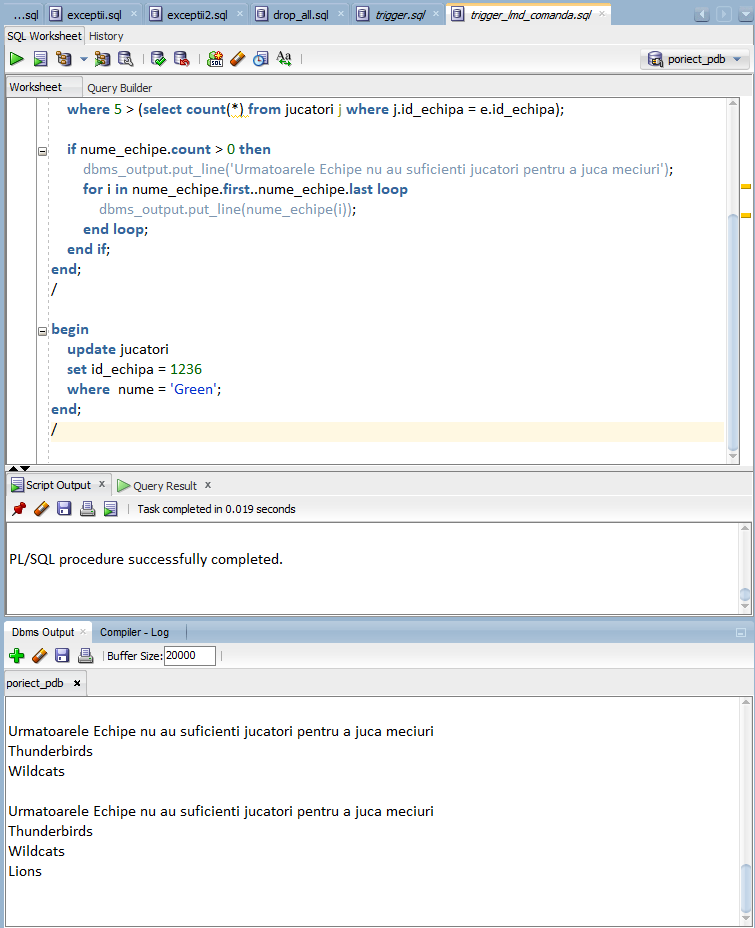
\includegraphics[width=40em, keepaspectratio]{trigger_lmd_comanda}
\pagebreak

\section{Problemă - Trigger LMD la nivel de linie}
	Definiți un trigger de tip LMD la nivel de linie. Declanșați trigger-ul.
\subsection{Cerință}
Să se definească un trigger pentru următoarea constrângere:
\begin{itemize}
	\item Să nu existe mai mult de 30 de etape într-un sezon, și să nu existe două etape într-un sezon cu același număr.
\end{itemize}
\subsection{Rezolvare}
\begin{lstlisting}
create or replace trigger verifica_max30etape_sezon
before insert on etape
for each row
declare
nr_etape number := 0;

etapa etape%rowtype;
begin
select count(*) into nr_etape
from etape 
where id_sezon = :new.id_sezon;

if nr_etape >= 30 then
raise_application_error(-20001, 'Nu poate fi adaugata etapa deoarece sezonul contine deja numarul maxim (30)');
end if;

select * into etapa
from etape
where id_sezon = :new.id_sezon and numar = :new.numar;

if etapa.id_etapa is not null then
raise_application_error(-20000, 'Nu poate fi adaugata etapa deoarece sezonul contine o etapa cu acelasi numar');
end if;

exception
when no_data_found then
nr_etape := 0;
end;
/

-- max 30
insert into etape values (1, 1000, 1); 

-- etapa cu acelasi numar
insert into sezoane values (10000, '', '');
insert into etape values(10016, 10000, 6);
insert into etape values(10015, 10000, 6);




\end{lstlisting}
\subsection{Captură de Ecran}
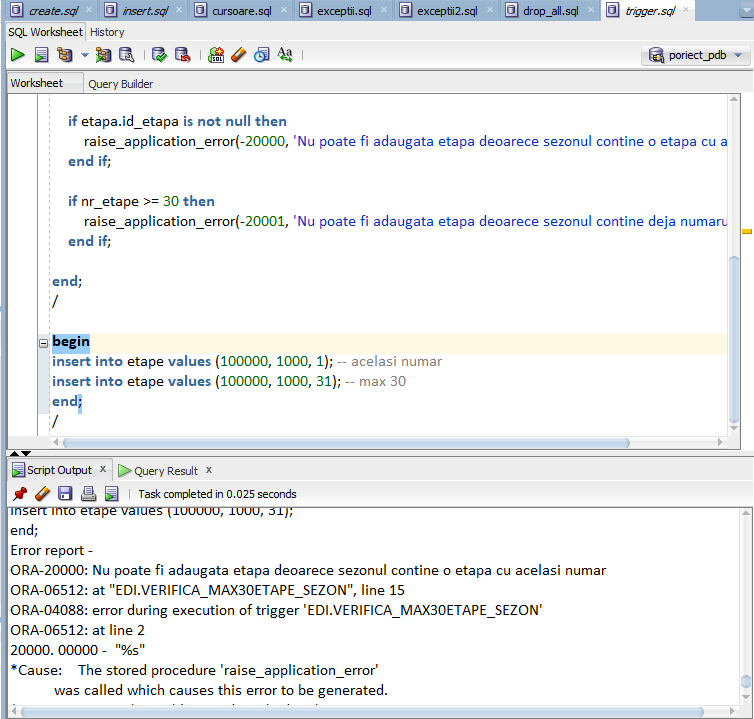
\includegraphics[width=40em, keepaspectratio]{trigger_lmd_linie}
\pagebreak


\section{Problema - Trigger LDD}
	Definiți un trigger de tip LDD. Declanșați trigger-ul.
\subsection{Cerință}
Să se definească un trigger care să împiedice adăugarea, ștergerea sau modificarea tabelelor dacă există un sezon în derulare în acel moment.
\subsection{Rezolvare}
\begin{lstlisting}
create or replace trigger fara_modificari_sezon_derulare
before ddl
on schema
declare 
sezon sezoane%rowtype;
begin
select * into sezon
from sezoane
where data_incepere < sysdate and sysdate < data_finalizare;

if sezon.id_sezon is not null then
raise_application_error(-20002, 'Nu se pot face modificare a structurii bazei de date in timpul unui sezon');
else
dbms_output.put_line('Modificari efectuate cu succes!');
end if;
exception
when no_data_found then
dbms_output.put_line('Modificari efectuate cu succes!');
--    when  others then
--            dbms_output.put_line('Eroare!');
end;
/


-- Pentru a avea un sezon in derulare
update sezoane
set data_finalizare = '10-JUN-24' 
where data_finalizare = '10-JUN-23';

alter table jucatori 
add  temp number;



\end{lstlisting}
\subsection{Captură de Ecran}
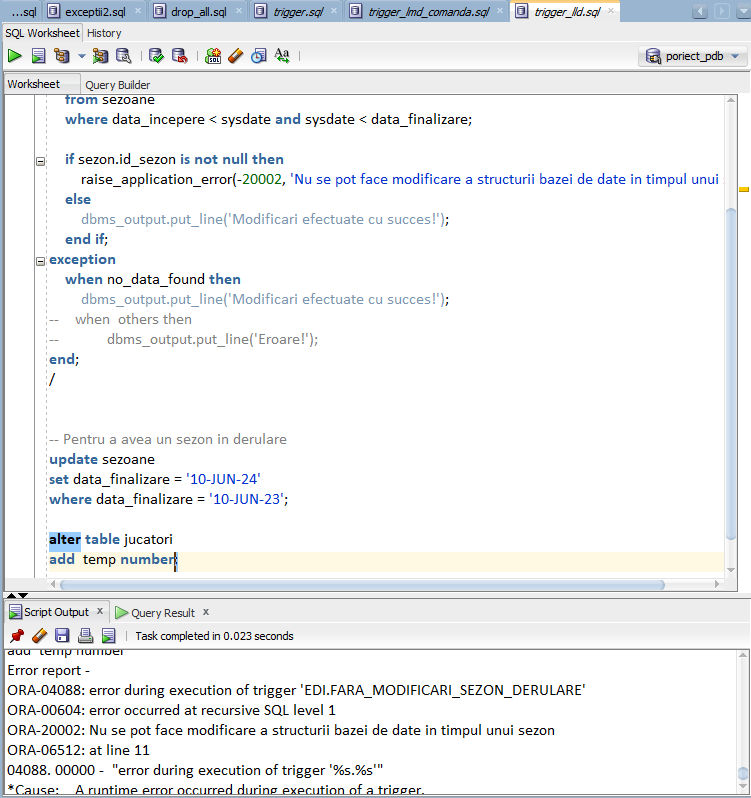
\includegraphics[width=40em, keepaspectratio]{trigger_ldd}
\pagebreak
\section{Opțional - Definire Pachet 1}
	Definiți un pachet care să conțină toate obiectele definite în cadrul proiectului. 
\subsection{Cod SQL}
\begin{multicols}{2}
\begin{lstlisting}
create or replace package pachet as 
function get_id return number;
function prenume_aleator return varchar2;
function nume_aleator return varchar2;

procedure sterge_date;
procedure insert_sezoane;
procedure insert_etape;
procedure insert_antrenori;
procedure insert_preparatori;
procedure insert_nutritionisti;
procedure insert_locatii;
procedure insert_arene;
procedure insert_echipe;
procedure insert_jucatori;
procedure insert_echipe_medicale;
procedure insert_meciuri;
procedure insert_arbitri;
procedure insert_comentatori;
procedure insert_statistici;
procedure insert_premii;
procedure insert_participari;
procedure insert_comentarii;
procedure insert_arbitraje;
procedure insert_distinctii;
procedure verifica_inserare;

procedure efectueaza_inserare;
procedure ex6_colectii;
procedure ex7_cursoare;

function ex8_exceptii(p_prenume in varchar2, p_salariu_minim in number) return number;
procedure ex9_exceptii (p_nume in angajati.nume%type);
end pachet;
/

create or replace package body pachet as
function get_id    
return number is
f_id number;
begin
select idseq.nextval into f_id
from dual;
return f_id;
end get_id;

function prenume_aleator
return varchar2 as 
prenume  varchar2(20);  
type StringArray is varray(20) of varchar2(20);
lista_prenume StringArray := StringArray(
'Ethan', 'Isaac', 'Leo', 'Miles', 'Asher',
'Maxwell', 'Oscar', 'Dylan', 'Oliver', 'Harrison',
'Nathan', 'Gabriel', 'Jasper', 'Ezra', 'Silas',
'Sebastian', 'Caleb', 'Gideon', 'Wyatt', 'Finn'
);
begin
prenume := lista_prenume(dbms_random.value(1, lista_prenume.last));
return prenume;
end prenume_aleator;

function nume_aleator
return varchar2 as 
nume  varchar2(20);  
type StringArray is varray(50) of varchar2(20);
lista_nume StringArray := StringArray('Smith', 'Johnson', 'Williams', 'Jones', 'Brown', 
'Davis', 'Miller', 'Wilson', 'Moore', 'Taylor', 'Anderson', 'Thomas', 'Jackson',
'White', 'Harris', 'Martin', 'Thompson', 'Garcia', 'Martinez', 'Robinson', 'Clark', 
'Rodriguez', 'Lewis', 'Lee', 'Walker', 'Hall', 'Allen', 'Young', 'Hernandez', 'King', 
'Wright', 'Lopez', 'Hill', 'Scott', 'Green', 'Adams', 'Baker', 'Gonzalez', 'Nelson',
'Carter', 'Mitchell', 'Perez', 'Roberts', 'Turner', 'Phillips', 'Campbell', 'Parker', 'Evans', 'Edwards');


begin
nume := lista_nume(dbms_random.value(1, lista_nume.last));
return nume;
end nume_aleator;

procedure sterge_date is 
begin
delete from arbitraje;
delete from comentarii;
delete from distinctii;
delete from participari;


delete from premii;
delete from statistici;

delete from arbitrii;
delete from comentatori;
delete from meciuri;
delete from echipe_medicale;

delete from jucatori;
delete from echipe;
delete from arene;
delete from locatii;

delete from preparatori_fizici;
delete from nutritionisti;
delete from antrenori;
delete from angajati;

delete from etape;
delete from sezoane;
end sterge_date;

procedure insert_sezoane is 
v_numar_sezoane number := 5;
v_format_data varchar2(11) := 'dd-mon-yyyy';
v_data_start date := to_date('15-aug-2022',v_format_data);
v_data_final date := to_date('10-jun-2023', v_format_data);
sezon sezoane%rowtype;
begin
sezon.data_incepere := v_data_start;
sezon.data_finalizare := v_data_final;
sezon.id_sezon := get_id();
for cnt in 1..v_numar_sezoane
loop
insert into sezoane
values sezon;
sezon.data_incepere := add_months(sezon.data_incepere, -12);
sezon.data_finalizare := add_months(sezon.data_finalizare, -12);
sezon.id_sezon := get_id();
end loop;

dbms_output.put_line('insert_sezoane OK');
end insert_sezoane;

procedure insert_etape is
v_numar_etape number := 30;
type id_sezoane is table of sezoane.id_sezon%type index by pls_integer;
v_id_sezoane id_sezoane; 
v_etapa etape%rowtype;
begin
select id_sezon
bulk collect into v_id_sezoane
from sezoane;

for cnt_sezon in v_id_sezoane.first..v_id_sezoane.last
loop
for cnt_etapa in 1..v_numar_etape
loop
v_etapa.id_etapa := get_id();
v_etapa.id_sezon := v_id_sezoane(cnt_sezon);
v_etapa.numar := cnt_etapa;
insert into etape
values v_etapa;
end loop;
end loop;
dbms_output.put_line('insert_etape OK');
end insert_etape;

procedure insert_antrenori is
numar_antrenori number := 16;
angajat angajati%rowtype;
antrenor antrenori%rowtype;
begin
for i in 1..numar_antrenori
loop
angajat.id_angajat := get_id();
angajat.nume := nume_aleator();
angajat.prenume := prenume_aleator();
angajat.salariu  := 100 * dbms_random.value(100, 200);
antrenor.id_angajat := angajat.id_angajat;

insert into angajati values angajat;
insert into antrenori values antrenor;
end loop;
dbms_output.put_line('insert_antrenori OK');
end insert_antrenori;

procedure insert_preparatori is
numar_preparatori number := 16;
angajat angajati%rowtype;
preparator preparatori_fizici%rowtype;
begin
for i in 1..numar_preparatori
loop
angajat.id_angajat := get_id();
angajat.nume := nume_aleator();
angajat.prenume := prenume_aleator();
angajat.salariu  := 100 * dbms_random.value(100, 200);
preparator.id_angajat := angajat.id_angajat;

insert into angajati values angajat;
insert into preparatori_fizici values preparator;
end loop;
dbms_output.put_line('insert_preparatori OK');
end insert_preparatori;

procedure insert_nutritionisti is
numar_nutritionisti number := 16;
angajat angajati%rowtype;
nutritionist nutritionisti%rowtype;
begin
for i in 1..numar_nutritionisti
loop
angajat.id_angajat := get_id();
angajat.nume := nume_aleator();
angajat.prenume := prenume_aleator();
angajat.salariu  := 100 * dbms_random.value(100, 200);
nutritionist.id_angajat := angajat.id_angajat;

insert into angajati values angajat;
insert into nutritionisti values nutritionist;
end loop;
dbms_output.put_line('insert_nutritionisti OK');
end insert_nutritionisti;

procedure insert_locatii is
type StringArray is varray(16) of varchar2(30);
orase StringArray := StringArray('New York City', 'Los Angeles','Las Vegas',
'Chicago', 'San Francisco', 'Miami', 'Orlando', 'Houston','Seattle', 
'Washington D.C.', 'Boston', 'Atlanta', 'Dallas', 'Denver',  
'New Orleans', 'San Diego');
strazi StringArray := StringArray('Fifth Avenue', 'Hollywood Boulevard', 
'Las Vegas Boulevard', 'Michigan Avenue', 'Lombard Street', 
'Ocean Drive', 'International Drive', 'NASA Road 1', 'Pike Place Market', 
'1600 Pennsylvania Avenue NW', 'Fenway Park',  'Peachtree Street', 
'Dealey Plaza', '16th Street Mall', 'Bourbon Street', 'Balboa Park');
locatie locatii%rowtype;
nr_locatii number := 16;
begin
for i in 1..nr_locatii
loop
locatie.id_locatie := get_id();
locatie.tara := 'USA';
locatie.oras := orase(i);
locatie.strada := strazi(i);
locatie.nr := dbms_random.value(100, 1000);
insert into locatii values locatie;
end loop;
dbms_output.put_line('insert_locatii OK');
end insert_locatii;

procedure insert_arene is
type IdLocatii is table of locatii.id_locatie%type index by pls_integer;
id_locatii IdLocatii;
numar_arene number := 16;
type StringArray is varray(16) of varchar2(30);
lista_arene StringArray := StringArray('The Thunderdome', 'The Coliseum', 'The Pit', 
'The Garden',  'The Staples Center', 'The Oracle', 'The Hoop House', 'The Den',
'The Arena', 'The Thunderdome', 'The Dome', 'The Palace',
'The Madhouse', 'The Pavilion', 'The Buzzer Beater', 'The Swish Center');
arena arene%rowtype;
begin
select id_locatie
bulk collect into id_locatii
from locatii;

for i in 1..numar_arene
loop
arena.id_arena := get_id();
arena.id_locatie := id_locatii(i);
arena.nume := lista_arene(i);
arena.locuri := 1000 * dbms_random.value(10, 20);

insert into arene values arena;
end loop;
dbms_output.put_line('insert_arene OK');
end insert_arene;

procedure insert_echipe is
type StringArray is varray(16) of varchar2(20);
lista_nume StringArray := StringArray('Lightning Bolts', 'Thunderbirds', 
'Wildcats', 'Heatwave', 'Hurricanes', 'Jaguars', 'Patriots', 'Titans',
'Vikings', 'Dragons', 'Raptors', 'Warriors',
'Hornets', 'Sharks', 'Lions', 'Knights');

type IdTable is table of number index by pls_integer;
id_arene IdTable;
id_antrenori IdTable;
id_preparatori IdTable;
id_nutritionisti IdTable;
echipa echipe%rowtype;
numar_echipe number := 16;
begin
select id_arena bulk collect into id_arene from arene;
select id_angajat bulk collect into id_antrenori from antrenori;
select id_angajat bulk collect into id_preparatori from preparatori_fizici;
select id_angajat bulk collect into id_nutritionisti from nutritionisti;

for i in 1..numar_echipe
loop
echipa.id_echipa := get_id();
echipa.id_arena := id_arene(i);
echipa.id_antrenor := id_antrenori(i);
echipa.id_preparator := id_preparatori(i);
echipa.id_nutritionist := id_nutritionisti(i);
echipa.nume := lista_nume(i);
echipa.an_infiintare := 1960 + dbms_random.value(0, 30);

insert into echipe values echipa;
end loop;
dbms_output.put_line('insert_echipe OK');
end insert_echipe;    

procedure insert_jucatori is 
type IdArray is table of echipe.id_echipa%type index by pls_integer;
id_echipe IdArray;
id_echipa echipe.id_echipa%type;
jucator jucatori%rowtype;
numar_jucatori_per_echipa number := 5;
begin
select id_echipa bulk collect into id_echipe from echipe;

for i in id_echipe.first..id_echipe.last
loop
id_echipa := id_echipe(i);
for i in 1..numar_jucatori_per_echipa
loop
jucator.id_jucator := get_id();
jucator.id_echipa := id_echipa;
jucator.nume := nume_aleator();
jucator.prenume := prenume_aleator();
jucator.inaltime := dbms_random.value(1.80, 2.25);
jucator.salariu := 1000 * dbms_random.value(40, 100);

insert into jucatori values jucator;
end loop;
end loop;

dbms_output.put_line('insert_jucatori OK');
end insert_jucatori;

procedure insert_echipe_medicale is
numar_echipe_medicale number := 5;
begin
for i in 1..numar_echipe_medicale
loop 
insert into echipe_medicale values(get_id());
end loop;

dbms_output.put_line('insert_echipe_medicale OK');
end insert_echipe_medicale;

procedure insert_meciuri is
type IdArray is table of number index by pls_integer;
id_sezoane IdArray;
id_echipe IdArray;
id_echipe_med IdArray;
id_etape IdArray;
meci meciuri%rowtype;
type IntArray is varray(8) of number;
x1 IntArray := IntArray(1, 2, 3, 4, 5, 6, 7, 8);
x2 IntArray := IntArray(16, 15, 14, 13, 12, 11, 10, 9);
rev boolean := false;
id_gazda number;
id_oaspete number;
temp number;
ids sezoane.id_sezon%type;
begin
select id_sezon bulk collect into id_sezoane from sezoane;
select id_echipa bulk collect into id_echipe from echipe;
select id_echipa_medicala bulk collect into id_echipe_med from echipe_medicale;



for i in id_sezoane.first..id_sezoane.last
loop
ids := id_sezoane(i);
select id_etapa bulk collect into id_etape 
from etape
where id_sezon = ids;

for nr_etapa in 1..30
loop
for i in 1..8
loop
if rev = false
then 
id_gazda := id_echipe(x1(i));
id_oaspete := id_echipe(x2(i));
else
id_gazda := id_echipe(x2(i));
id_oaspete := id_echipe(x1(i));
end if;

meci.id_meci := get_id();
meci.id_etapa := id_etape(nr_etapa);
meci.id_echipa_gazda := id_gazda;
meci.id_echipa_oaspete := id_oaspete;
meci.id_echipa_medicala := id_echipe_med(dbms_random.value(1, id_echipe_med.last));
meci.scor_gazda := dbms_random.value(60, 100);
meci.scor_oaspete := meci.scor_gazda + (dbms_random.value(0, 94) - 47);

insert into meciuri values meci;

end loop;
temp := x2(1);
for i in 1..7
loop
x2(i) := x2(i+1);
end loop;
x2(8) := x1(8);
for i in reverse 3..8
loop
x1(i) := x1(i-1);
end loop;
x1(2) := temp;

if x1(2) = 2
then rev := true;
end if;

end loop;
end loop;
end insert_meciuri;    

procedure insert_arbitri is
arbitru arbitrii%rowtype;
numar_arbitrii number := 50;
begin
for i in 1..numar_arbitrii
loop
arbitru.nume := nume_aleator();
arbitru.prenume := prenume_aleator();
arbitru.id_arbitru := get_id();
arbitru.data_obtinere_licenta := to_date(trunc(
dbms_random.value(to_char(date '1990-01-01','J') ,to_char(date '2015-12-31','J') )
),'J' );
insert into arbitrii values arbitru;
end loop;

dbms_output.put_line('insert_arbitrii OK');
end insert_arbitri;

procedure insert_comentatori is
comentator comentatori%rowtype;
numar_comentatori number := 10;
begin
for i in 1..numar_comentatori
loop
comentator.nume := nume_aleator();
comentator.prenume := prenume_aleator();
comentator.id_comentator := get_id();
insert into comentatori values comentator;
end loop;

dbms_output.put_line('insert_comentatori OK');
end insert_comentatori;

procedure insert_statistici is
type IdArray is table of number index by pls_integer;
id_meciuri IdArray;
id_jucatori IdArray;
statistica statistici%rowtype;
meci meciuri%rowtype;
idm meciuri.id_meci%type;
idj jucatori.id_jucator%type;
begin
select id_meci bulk collect into id_meciuri from meciuri;

for i in id_meciuri.first..id_meciuri.last
loop
idm := id_meciuri(i);
select * into meci from meciuri where id_meci = idm;
select id_jucator bulk collect into id_jucatori
from jucatori
where id_echipa = meci.id_echipa_gazda or id_echipa = meci.id_echipa_oaspete;

for j in id_jucatori.first..id_jucatori.last
loop
idj := id_jucatori(j);
statistica.id_statistica := get_id();
statistica.id_meci := idm;
statistica.id_jucator := idj;
statistica.minute_jucate := dbms_random.value(20, 48);
statistica.aruncari_2pct := dbms_random.value(0, 30);
statistica.aruncari_2pct_marcate := dbms_random.value(0, statistica.aruncari_2pct);
statistica.aruncari_3pct := dbms_random.value(0, 20);
statistica.aruncari_3pct_marcate := dbms_random.value(0, statistica.aruncari_3pct);
statistica.aruncari_libere := dbms_random.value(0, 10);
statistica.aruncari_libere_marcate := dbms_random.value(0, statistica.aruncari_libere);
statistica.pase_decisive := dbms_random.value(0, 25);
statistica.recuperari := dbms_random.value(0,15);
statistica.faulturi := dbms_random.value(0, 5);

insert into statistici values statistica;
end loop;
end loop;

dbms_output.put_line('insert_statistica OK');
end insert_statistici;

procedure insert_premii is
type StringArray is varray(5) of varchar2(50);
lista_premii StringArray := StringArray('Most Valuable Player (MVP)', 
'Team Player of the Year',
'Defensive Player of the Year', 'Sportsmanship Award', 'Best Distance Shooter');
premiu premii%rowtype;
begin
for i in lista_premii.first..lista_premii.last
loop
premiu.id_premiu := get_id();
premiu.denumire := lista_premii(i);
insert into premii values premiu;
end loop;

dbms_output.put_line('inser_premii OK');
end insert_premii;

procedure insert_participari is
type IdArray is table of number index by pls_integer;
id_sezoane IdArray;
id_echipe IdArray;
participare participari%rowtype;
ids sezoane.id_sezon%type;
ide echipe.id_echipa%type;
begin
select id_sezon bulk collect into id_sezoane from sezoane;
select id_echipa bulk collect into id_echipe from echipe;

for i in id_sezoane.first..id_sezoane.last
loop
ids := id_sezoane(i);
for j in id_echipe.first..id_echipe.last
loop
ide := id_echipe(j);
participare.id_sezon := ids;
participare.id_echipa := ide;
insert into participari values participare;
end loop;
end loop;

dbms_output.put_line('insert_participari OK');
end insert_participari;

procedure insert_comentarii is
comentariu comentarii%rowtype;
type IdArray is table of number index by pls_integer;
id_meciuri IdArray;
id_comentatori IdArray;
a number(2,0);
b number(2,0);
c number(2,0);
begin
select id_meci bulk collect into id_meciuri from meciuri;
select id_comentator bulk collect into id_comentatori from comentatori;

for i in id_meciuri.first..id_meciuri.last
loop
a := dbms_random.value(1,id_comentatori.last);
b := dbms_random.value(1,id_comentatori.last);
c := dbms_random.value(1,id_comentatori.last);
while a = b
loop
b := dbms_random.value(1,id_comentatori.last);
end loop;
while a = c or b = c
loop
c := dbms_random.value(1,id_comentatori.last);
end loop;
comentariu.id_meci := id_meciuri(i);
comentariu.id_comentator := id_comentatori(a);
insert into comentarii values comentariu;
comentariu.id_comentator := id_comentatori(b);
insert into comentarii values comentariu;
comentariu.id_comentator := id_comentatori(c);
insert into comentarii values comentariu;
end loop;

dbms_output.put_line('insert-comentarii OK');
end insert_comentarii;

procedure insert_arbitraje is
arbitraj arbitraje%rowtype;
type IdArray is table of number index by pls_integer;
id_meciuri IdArray;
id_arbitrii IdArray;
a number(2,0);
b number(2,0);
c number(2,0);
begin
select id_meci bulk collect into id_meciuri from meciuri;
select id_arbitru bulk collect into id_arbitrii from arbitrii;

for i in id_meciuri.first..id_meciuri.last
loop
a := dbms_random.value(1,id_arbitrii.last);
b := dbms_random.value(1,id_arbitrii.last);
c := dbms_random.value(1,id_arbitrii.last);
while a = b
loop
b := dbms_random.value(1,id_arbitrii.last);
end loop;
while a = c or b = c
loop
c := dbms_random.value(1,id_arbitrii.last);
end loop;
arbitraj.id_meci := id_meciuri(i);
arbitraj.id_arbitru := id_arbitrii(a);
insert into arbitraje values arbitraj;
arbitraj.id_arbitru := id_arbitrii(b);
insert into arbitraje values arbitraj;
arbitraj.id_arbitru := id_arbitrii(c);
insert into arbitraje values arbitraj;
end loop;

dbms_output.put_line('insert-arbitraje OK');
end insert_arbitraje;

procedure insert_distinctii is
distinctie distinctii%rowtype;
type IdArray is table of number index by pls_integer;
id_sezoane IdArray;
id_jucatori IdArray;
id_premii IdArray;
begin
select id_sezon bulk collect into id_sezoane from sezoane;
select id_jucator bulk collect into id_jucatori from jucatori;
select id_premiu bulk collect into id_premii from premii;

for i in id_sezoane.first..id_sezoane.last
loop
for j in id_premii.first..id_premii.last
loop
distinctie.id_sezon := id_sezoane(i);
distinctie.id_premiu := id_premii(j);
distinctie.id_jucator := id_jucatori(dbms_random.value(1, id_jucatori.last));

insert into distinctii values distinctie;
end loop;
end loop;

dbms_output.put_line('insert_distinctii OK');
end insert_distinctii;

procedure verifica_inserare is
cnt number;
type StringArray is varray(20) of varchar2(20);
tabele StringArray := StringArray('angajati', 'antrenori', 'arbitrii', 
'arene', 'comentarii', 'comentatori', 'distinctii', 'echipe', 
'echipe_medicale', 'etape', 'jucatori', 'locatii', 
'meciuri', 'nutritionisti', 'participari', 'premii', 'preparatori_fizici', 
'sezoane', 'statistici');
begin
select count(*) into cnt from angajati;
dbms_output.put_line('Exista ' || cnt || ' angajati.');
select count(*) into cnt from antrenori;
dbms_output.put_line('Exista ' || cnt || ' antrenori.');   
select count(*) into cnt from arbitraje;
dbms_output.put_line('Exista ' || cnt || ' arbitraje.');
select count(*) into cnt from arbitrii;
dbms_output.put_line('Exista ' || cnt || ' arbitrii.');
select count(*) into cnt from arene;
dbms_output.put_line('Exista ' || cnt || ' arene.');
select count(*) into cnt from comentarii;
dbms_output.put_line('Exista ' || cnt || ' comentarii.');   
select count(*) into cnt from comentatori;
dbms_output.put_line('Exista ' || cnt || ' comentatori.');   
select count(*) into cnt from distinctii;
dbms_output.put_line('Exista ' || cnt || ' distinctii.');
select count(*) into cnt from echipe;
dbms_output.put_line('Exista ' || cnt || ' echipe.');
select count(*) into cnt from echipe_medicale;
dbms_output.put_line('Exista ' || cnt || ' echipe_medicale.');
select count(*) into cnt from etape;
dbms_output.put_line('Exista ' || cnt || ' etape.');   
select count(*) into cnt from jucatori;
dbms_output.put_line('Exista ' || cnt || ' jucatori.');
select count(*) into cnt from locatii;
dbms_output.put_line('Exista ' || cnt || ' locatii.');
select count(*) into cnt from meciuri;
dbms_output.put_line('Exista ' || cnt || ' meciuri.');
select count(*) into cnt from nutritionisti;
dbms_output.put_line('Exista ' || cnt || ' nutritionisti.');   
select count(*) into cnt from participari;
dbms_output.put_line('Exista ' || cnt || ' participari.');
select count(*) into cnt from premii;
dbms_output.put_line('Exista ' || cnt || ' premii.');
select count(*) into cnt from preparatori_fizici;
dbms_output.put_line('Exista ' || cnt || ' preparatori_fizici.');   
select count(*) into cnt from sezoane;
dbms_output.put_line('Exista ' || cnt || ' sezoane.');
select count(*) into cnt from statistici;
dbms_output.put_line('Exista ' || cnt || ' statistici.');

end verifica_inserare;

procedure efectueaza_inserare is
begin
sterge_date();
insert_sezoane();
insert_etape();
insert_antrenori();
insert_preparatori();
insert_nutritionisti();
insert_locatii();
insert_arene();
insert_echipe();
insert_jucatori();
insert_echipe_medicale();
insert_meciuri();
insert_arbitri();
insert_comentatori();
insert_statistici();
insert_premii();
insert_participari();
insert_comentarii();
insert_arbitraje();
insert_distinctii();
verifica_inserare();
end efectueaza_inserare;

procedure ex6_colectii is
-- Am ales tabloul imbricat deoarece numarul de sezoane este necunoscut 
-- si nu fac stergeri pe parcursul programului
type IdSezoane is table of sezoane.id_sezon%type ;
id_sezoane IdSezoane;
id_sezon_curent sezoane.id_sezon%type;

-- Am ales varray deoarece stiu dinainte numarul de etape (30) dintr-un sezon,
-- respectiv numarul de meciuri dintr-o etapa (8), si nu fac stergeri in aceasta colectie
type IdEtape is varray(30) of etape.id_etapa%type;
id_etape IdEtape;
id_etapa_curenta sezoane.id_sezon%type;

type RecordJucator is record
(
id_jucator jucatori.id_jucator%type,
puncte number
);
type idJucatoriTop3 is varray(3) of RecordJucator;
id_jucatori_3 IdJucatoriTop3;
rec RecordJucator;

-- Am ales tablou indexat deoarece indicii vor fi anumite id-uri ale jucatorilor, nu neaparat dense.
type TabelPuncteJucatori is table of number(4) index by pls_integer;
puncte_jucator TabelPuncteJucatori := TabelPuncteJucatori();

nr_etape number; -- restriciile spun ca pentru fiecare sezon exista 30 etape

maxim number;
id_mvp jucatori.id_jucator%type;
jucator jucatori%rowtype;

begin
select id_sezon bulk collect into id_sezoane from sezoane;

for it_sezon in id_sezoane.first..id_sezoane.last loop
id_sezon_curent := id_sezoane(it_sezon);
select count(id_etapa) collect into nr_etape 
from etape
where id_sezon = id_sezon_curent;

if nr_etape != 30
then 
dbms_output.put_line ('In sezonul ' || id_sezon_curent || 
' nu sunt 30 de etape ( ' || nr_etape || ' )');
continue;
end if;

select id_etapa bulk collect into id_etape 
from etape
where id_sezon = id_sezon_curent;

puncte_jucator := TabelPuncteJucatori();
maxim := 0;
for it_etapa in id_etape.first..id_etape.last loop
id_etapa_curenta := id_etape(it_etapa);
with jucatori_si_puncte as
(select j.id_jucator, 2 * aruncari_2pct_marcate + 3 * aruncari_3pct_marcate + aruncari_libere_marcate
from jucatori j
join meciuri m on m.id_etapa = id_etapa_curenta and
((m.id_echipa_gazda = j.id_echipa and scor_gazda >  scor_oaspete ) or
(m.id_echipa_oaspete = j.id_echipa and scor_gazda <  scor_oaspete ))
join statistici s on s.id_meci = m.id_meci and s.id_jucator = j.id_jucator
order by 2 desc)
select * bulk collect into id_jucatori_3
from jucatori_si_puncte
where rownum <= 3;

for it in id_jucatori_3.first..id_jucatori_3.last loop
rec := id_jucatori_3(it);
if puncte_jucator.exists(rec.id_jucator) = false
then puncte_jucator(rec.id_jucator) := 0;
end if;

puncte_jucator(rec.id_jucator) := puncte_jucator(rec.id_jucator) + rec.puncte;
if maxim < puncte_jucator(rec.id_jucator)
then
maxim := puncte_jucator(rec.id_jucator);
id_mvp := rec.id_jucator;
end if;
end loop;
end loop;

select * into jucator
from jucatori
where id_jucator = id_mvp;

dbms_output.put_line(jucator.nume || ' ' || jucator.prenume || '  id: ' || id_mvp || ' puncte:  ' || puncte_jucator(id_mvp));

end loop;

end ex6_colectii;

procedure ex7_cursoare is
cursor c_id_arbitri (idm meciuri.id_meci%type) is
select id_arbitru from arbitraje where arbitraje.id_meci = idm;


type IdArbitri is table of arbitrii.id_arbitru%type;
id_arbitri IdArbitri;
arbitru arbitrii%rowtype;

cursor meciuriVerificate is
select *
from meciuri
where abs(scor_gazda - scor_oaspete) =  
(select max(abs(scor_gazda - scor_oaspete))
from meciuri);

cursor arbitriVerificati (idm meciuri.id_meci%type) is
select *
from arbitrii
where id_arbitru in (select id_arbitru from arbitraje where arbitraje.id_meci = idm);

cursor jucatoriMeci (
id_gazda echipe.id_echipa%type,
id_oaspete echipe.id_echipa%type, 
nume_arbitru arbitrii.nume%type) is
select id_jucator , nume, prenume, id_echipa
from jucatori 
where (id_echipa = id_gazda or id_echipa = id_oaspete)
and jucatori.nume = nume_arbitru;

mesaj varchar2(50);
id_echipa echipe.id_Echipa%type;
begin

-- CICLU CURSOR
for meci in meciuriVerificate loop
--        dbms_output.put_line('meci: ' || meci.id_meci);

-- CURSOR CLASIC PARAMETRIZAT
open c_id_arbitri(meci.id_meci);
fetch c_id_arbitri bulk collect into id_arbitri;
close c_id_arbitri;

for i in id_arbitri.first..id_arbitri.last loop
select * into arbitru
from arbitrii
where id_arbitru = id_arbitri(i);
--            dbms_output.put_line('arbitru: ' || arbitru.id_arbitru);
-- CICLU CURSOR PARAMETRIZAT
for jucator in jucatoriMeci(meci.id_echipa_gazda, meci.id_echipa_oaspete, arbitru.nume) loop

if meci.scor_gazda > meci.scor_oaspete
then id_echipa := meci.id_echipa_gazda;
else id_echipa := meci.id_echipa_oaspete;
end if;

if jucator.id_echipa = id_echipa
then mesaj := ' (Victorie)';
else mesaj := ' (Infrangere)';
end if;

dbms_output.put_line(meci.id_meci || ': ' ||
arbitru.id_arbitru || ' ' || arbitru.nume || ' ' || arbitru.prenume || ' - ' ||
jucator.id_jucator || ' ' || jucator.nume || ' ' || jucator.prenume || ' - ' || 
meci.scor_gazda || '-' || meci.scor_oaspete || mesaj);

end loop;
end loop;
end loop;

end;

function ex8_exceptii
(p_prenume in varchar2,
p_salariu_minim in number)
return number
is
ex_no_first_name exception;
ex_no_salary exception;
type RecordEchipa is Record (
--        id_echipa echipe.id_echipa%type,
nume varchar2(50),
suma_salarii number
);
type ListaEchipe is table of RecordEchipa;
lista_echipe ListaEchipe;

aux number := 0;

begin
select count(*) collect into aux
from (select id_jucator from jucatori where lower(prenume) like lower(p_prenume)
union select id_angajat from angajati where lower(prenume) like lower(p_prenume));

if aux = 0 then
raise ex_no_first_name;
end if;

with persoane as (
select e.id_echipa id_echipa, salariu 
from angajati a
join echipe e on e.id_antrenor = a.id_angajat or e.id_preparator = a.id_angajat 
or e.id_nutritionist = a.id_angajat
where lower(a.prenume) like lower(p_prenume) and a.salariu >= p_salariu_minim
union
select id_echipa, salariu from jucatori
where lower(prenume) like lower(p_prenume) and salariu >= p_salariu_minim
)
select * bulk collect into lista_echipe
from (
select e.nume, sum(p.salariu) 
from persoane p
join echipe e on e.id_echipa = p.id_echipa
group by e.nume
)
order by 2 desc;


if lista_echipe.count = 0 then
raise ex_no_salary;
end if;

aux := 0;
for i in lista_Echipe.first..lista_echipe.last loop
dbms_output.put_line(lista_echipe(i).nume || ' - ' || lista_echipe(i).suma_salarii);
aux := aux + lista_echipe(i).suma_salarii;
end loop;

return aux;

exception
when ex_no_first_name then
dbms_output.put_line('Exceptie: nu exista prenumele ' || p_prenume);
return 0;
when ex_no_salary then
dbms_output.put_line('Exceptie: nu exista salarii mai mari decat ' || p_salariu_minim);
return 0;
when others then
dbms_output.put_line('Alta Exceptie');
return 0;
end ex8_exceptii;

procedure ex9_exceptii
(p_nume in angajati.nume%type
)
is
ex_no_player exception;
type RecAngajat is record (
nume angajati.nume%type, 
prenume angajati.prenume%type,
nume_echipa echipe.nume%type, 
post varchar2(20)
);
angajat RecAngajat;
type RecEchipa is record (
id echipe.id_echipa%type,
nume echipe.nume%type);
echipa RecEchipa;

type RecJucator is record(
id jucatori.id_jucator%type,
nume jucatori.nume%type, 
prenume jucatori.prenume%type, 
proc_3pct number(5, 2), 
proc_faulturi number(5, 2),
avg_pase number(5, 2)
);
type ListaJucatori is table of RecJucator;
lista_jucatori ListaJucatori;

begin

select a.nume, a.prenume, e.nume, (case
when a.id_angajat = e.id_antrenor then 'antrenor'
when a.id_angajat = e.id_preparator then 'preparator fizic'
when a.id_angajat = e.id_nutritionist then 'nutritionist'
end) post
into angajat
from angajati a, echipe e
where lower(a.nume) = lower(p_nume)
and id_angajat in (e.id_antrenor, e.id_preparator, e.id_nutritionist);

dbms_output.put_line(angajat.nume || ' ' || angajat.prenume || ' lucreaza pentru echipa ' || 
angajat.nume_echipa || ' pe postul de ' || angajat.post);

with info_echipa as (
select id_echipa, e.nume
from echipe e 
where (p_nume) in
(select nume
from angajati
where lower(nume) = lower(p_nume)
and id_angajat in (e.id_antrenor, e.id_preparator, e.id_nutritionist))
)
select j.id_jucator, j.nume, j.prenume, 100 * sum(s.aruncari_3pct_marcate) / sum(s.aruncari_3pct),
100 * sum(case when s.faulturi > 0 then 1 else 0 end) / count(*), avg(s.pase_decisive)
bulk collect into lista_jucatori
from jucatori j
join statistici s on s.id_jucator = j.id_jucator
where j.id_jucator in (select distinct id_jucator from distinctii)
and j.id_echipa = (select id_echipa from info_echipa)
group by (j.id_jucator, j.nume, j.prenume);

if lista_jucatori.count = 0 then
raise ex_no_player;
end if;

for i in lista_jucatori.first..lista_jucatori.last loop
dbms_output.put_line(lista_jucatori(i).nume || ' ' || lista_jucatori(i).prenume || ' -  procentaj 3pct: ' 
|| lista_jucatori(i).proc_3pct || '% - procentaj meciuri cu fault:  ' || lista_jucatori(i).proc_faulturi || 
'% - medie pase decisive: ' || lista_jucatori(i).avg_pase);
end loop;

exception
when no_data_found then
dbms_output.put_line('Nu exista niciun angajat cu numele ' || p_nume);
when too_many_rows then
dbms_output.put_line('Exista mai multi angajati cu numele ' || p_nume);
when ex_no_player then
dbms_output.put_line('Nu exista niciun jucator care sa fi primit vreo distinctie in echipa ' || angajat.nume_echipa);
end ex9_exceptii;



end pachet;
/
\end{lstlisting}
\end{multicols}

\pagebreak
\subsection{Exemplu Execuție}
\begin{lstlisting}
-- Din cauza faptului ca majoritatea datelor din baza de date sunt generate aleator, 
-- este posibil ca unele apeluri sa obtina rezultate diferite decat in capturile de ecran

begin
pachet.efectueaza_inserare();
pachet.ex6_colectii();
pachet.ex7_cursoare();

-- EX 8
dbms_output.put_line(pachet.ex8_exceptii('isaac', 50000));
dbms_output.put_line(pachet.ex8_exceptii('prenume', 1000));
dbms_output.put_line(pachet.ex8_exceptii('isaac', 100000));

-- EX 9
dbms_output.put_line('Apel cu numele: Johnson');
pachet.ex9_exceptii('Johnson');
dbms_output.put_line('Apel cu numele: Carter');
pachet.ex9_exceptii('Carter');
dbms_output.put_line('Apel cu numele: Clark');
pachet.ex9_exceptii('Clark');
dbms_output.put_line('Apel cu numele: John');
pachet.ex9_exceptii('John');
end;
/

\end{lstlisting}

\subsection{Captură de Ecran}
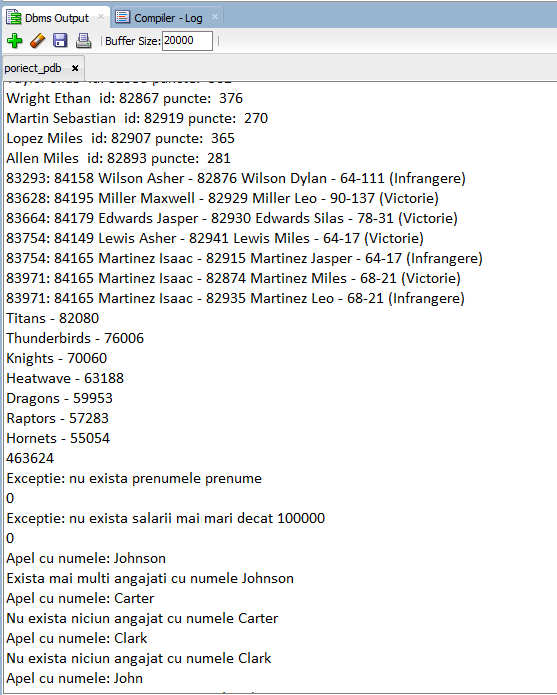
\includegraphics[width=40em, keepaspectratio]{pachet_executie}
\pagebreak

\section{Opțional - Definire Pachet 2}
	Definiți un pachet care să includă tipuri de date complexe și obiecte necesare unui flux de acțiuni
	integrate, specifice bazei de date definite (minim 2 tipuri de date, minim 2 funcții, minim 2 proceduri). 

\subsection{Cerinta}
La finalul unui sezon, asociatia de baschet doreste sa verifice daca toate datele corespunzatoare meciurilor din sezonul curent se afla in baza de date (toate etapele exista, iar fiecare echipa a jucat 30 de meciuri). In caz afirmativ, trebuie sa acorde cele 5 premii:
\begin{itemize}
	\item "Most Valuable Player (MVP)" - pentru jucatorul cu cele mai multe puncte inscrise
	\item "Team Player of the Year" - pentru jucatorul cu cele mai multe pase decisive
	\item "Defensive Player of the Year" - pentru jucatorul cu cele mai multe recuperari
	\item "Sportsmanship Award" - pentru jucatorul cu cele mai putine faulturi
	\item "Best Distance Shooter" - pentru jucatorul cu cele mai multe cosuri de 3 puncte inscrise
\end{itemize}
In caz de egalitate, comisia trebuie sa fie instiintata printr-un mesaj pentru a decide cine este premiat (nu se va adauga premiul in baza de date).
	
\subsection{Rezolvare}
\begin{multicols}{2}
\begin{lstlisting}
select * from premii;

create or replace package acordare_premii as
type StatisticiJucator is record (puncte number, pase number, recuperari number, faulturi number, cosuri3pct number);
type TabelStatistici is table of StatisticiJucator index by pls_integer;
statisticiSezon TabelStatistici := TabelStatistici();

ultimul_sezon_calculat number := -1; -- Id-ul sezonului pentru care s-au calculat statisticile ultima data.

function numeSiEchipaJucator(idj in number) return varchar2;

function verifica_sezon(an_incepere in number) return boolean;

procedure acorda_premii(an_incepere in number);

function obtine_statistici_jucator(idj in number, ids in number) return StatisticiJucator;

procedure calculeaza_statistici(ids number);


end acordare_premii;
/

create or replace package body acordare_premii as
function verifica_sezon(an_incepere in number)
return boolean as
ids number := 0;
nr_etape number := 0;
nr_meciuri number := 0;
type TabelIdEchipe is table of echipe.id_echipa%type;
id_echipe TabelIdEchipe;
begin
select id_sezon into ids
from sezoane s
where to_char(s.data_incepere, 'yyyy') = to_char(an_incepere);

if ids = 0 then
dbms_output.put_line('Sezonul nu exista');
return false;
end if;

select count(*) into nr_etape
from etape e
where e.id_sezon = ids;

if nr_etape != 30 then
dbms_output.put_line('Sezonul nu contine ' || nr_etape || ' etape in loc de 30');
return false;
end if;

select e.id_echipa bulk collect into id_echipe
from echipe e
where exists (select * from participari p where p.id_sezon = ids and p.id_echipa = e.id_echipa);

if id_echipe.count() != 16 then
dbms_output.put_line('Sezonul nu contine 16 echipe');
return false;
end if;

for i in id_echipe.first..id_echipe.last loop
select count(*) collect into nr_meciuri
from meciuri m 
where (m.id_echipa_oaspete = id_echipe(i) or m.id_echipa_gazda = id_echipe(i))
and ids = (select e.id_sezon from etape e join sezoane s on s.id_sezon = e.id_sezon where e.id_etapa = m.id_etapa);

if nr_meciuri != 30 then
dbms_output.put_line('Echipa cu id ' || id_echipe(i) || 'a jucat ' || nr_meciuri || ' in loc de 30');
return false;
end if;
end loop;

return true;
exception
when no_data_found then dbms_output.put_line('EX: NO DATA FOUND');
return false;
end verifica_sezon;

procedure acorda_premii(an_incepere in number)
as
aux number := 0;
maxim StatisticiJucator := StatisticiJucator(0, 0, 0, 100000, 0);
id_castigator StatisticiJucator := StatisticiJucator();
cnt StatisticiJucator := StatisticiJucator(0, 0, 0, 0, 0);
ids number := 0;
begin
dbms_output.put_line('Se incearca acordarea premiilor');
if verifica_sezon(an_incepere) = false then
dbms_output.put_line('Nu au fost acordate premiile');
return;
end if;

select id_sezon into ids
from sezoane s
where to_char(s.data_incepere, 'yyyy') = to_char(an_incepere);

if ids != ultimul_sezon_calculat then
calculeaza_statistici(ids);
end if;


for i in statisticiSezon.first..statisticiSezon.last loop
if maxim.puncte < statisticiSezon(i).puncte then 
maxim.puncte := statisticiSezon(i).puncte;
cnt.puncte := 1;
id_castigator.puncte := i;
elsif maxim.puncte = statisticiSezon(i).puncte then 
cnt.puncte := cnt.puncte + 1;
end if;

if maxim.pase < statisticiSezon(i).pase then 
maxim.pase := statisticiSezon(i).pase; 
cnt.pase := 1;
id_castigator.pase := i;
elsif maxim.pase = statisticiSezon(i).pase then 
cnt.pase :=  cnt.pase + 1;
end if;

if maxim.recuperari < statisticiSezon(i).recuperari then 
maxim.recuperari := statisticiSezon(i).recuperari; 
cnt.recuperari := 1;
id_castigator.recuperari := i;
elsif maxim.recuperari = statisticiSezon(i).recuperari then 
cnt.recuperari :=  cnt.recuperari + 1;
end if;

if maxim.faulturi > statisticiSezon(i).faulturi then 
maxim.faulturi := statisticiSezon(i).faulturi; 
cnt.faulturi := 1;
id_castigator.faulturi := i;
elsif maxim.faulturi = statisticiSezon(i).faulturi then 
cnt.faulturi :=  cnt.faulturi + 1;
end if;

if maxim.cosuri3pct < statisticiSezon(i).cosuri3pct then 
maxim.cosuri3pct := statisticiSezon(i).cosuri3pct; 
cnt.cosuri3pct := 1;
id_castigator.cosuri3pct := i;
elsif maxim.cosuri3pct = statisticiSezon(i).cosuri3pct then 
cnt.cosuri3pct := cnt.cosuri3pct + 1;
end if;

end loop;

delete from distinctii where id_sezon = ids;

if cnt.puncte = 1 then
dbms_output.put_line(numeSiEchipaJucator(id_castigator.puncte) || ' --- ' || 'Most Valuable Player (MVP)');
select id_premiu into aux from premii where denumire like  'Most Valuable Player (MVP)';
insert into distinctii values (ids, id_castigator.puncte, aux);
else
dbms_output.put_line('Sunt mai multi jucatori care pot castiga ' || 'Most Valuable Player (MVP)' );
end if;


if cnt.pase = 1 then
dbms_output.put_line(numeSiEchipaJucator(id_castigator.pase) || ' --- ' || 'Team Player of the Year');
select id_premiu into aux from premii where denumire like 'Team Player of the Year';
insert into distinctii values (ids, id_castigator.pase, aux);
else
dbms_output.put_line('Sunt mai multi jucatori care pot castiga ' || 'Team Player of the Year');
end if;       

if cnt.recuperari = 1 then
dbms_output.put_line(numeSiEchipaJucator(id_castigator.recuperari) || ' --- ' ||  'Defensive Player of the Year');
select id_premiu into aux from premii where denumire like  'Defensive Player of the Year';
insert into distinctii values (ids, id_castigator.recuperari, aux);
else
dbms_output.put_line('Sunt mai multi jucatori care pot castiga ' ||  'Defensive Player of the Year');
end if;

if cnt.faulturi = 1 then
dbms_output.put_line(numeSiEchipaJucator(id_castigator.faulturi) || ' --- ' || 'Sportsmanship Award');
select id_premiu into aux from premii where denumire like  'Sportsmanship Award';
insert into distinctii values (ids, id_castigator.faulturi, aux);
else
dbms_output.put_line('Sunt mai multi jucatori care pot castiga ' || 'Sportsmanship Award');
end if;

if cnt.cosuri3pct = 1 then
dbms_output.put_line(numeSiEchipaJucator(id_castigator.cosuri3pct) || ' --- ' || 'Best Distance Shooter');
select id_premiu into aux from premii where denumire like 'Best Distance Shooter';
insert into distinctii values (ids, id_castigator.cosuri3pct, aux);
else
dbms_output.put_line('Sunt mai multi jucatori care pot castiga ' || 'Best Distance Shooter');
end if;
--       dbms_output.put_line(maxim.puncte || ' ' || maxim.pase || ' ' ||  maxim.recuperari || ' ' || maxim.faulturi || ' ' || maxim.cosuri3pct);
--    dbms_output.put_line(cnt.puncte || ' ' || cnt.pase || ' ' ||  cnt.recuperari || ' ' || cnt.faulturi || ' ' || cnt.cosuri3pct);

dbms_output.put_line('S-au acordat premiile cu succes');
end acorda_premii;

function numeSiEchipaJucator(idj in number) return varchar2
is
str varchar2(50) := '';
begin
select j.nume || ' ' || j.prenume || ' - ' || e.nume into str
from jucatori j
join echipe e on e.id_echipa = j.id_echipa
where j.id_jucator = idj;

return str;
exception
when others then dbms_output.put_line('Eroare la obtinerea numelui si echipei unui jucator');
return '';
end numeSiEchipaJucator;

function obtine_statistici_jucator(idj in number, ids in number) return StatisticiJucator
as
statistica StatisticiJucator;
begin
select 2 * sum(s.aruncari_2pct_marcate) + 3 * sum(s.aruncari_3pct_marcate) + sum(s.aruncari_libere_marcate), 
sum(s.pase_decisive), 
sum(s.recuperari), 
sum(s.faulturi), 
sum(s.aruncari_3pct_marcate)
into statistica
from statistici s 
where s.id_jucator = idj and ids = (select e.id_sezon from etape e join meciuri m on m.id_etapa = e.id_etapa where s.id_meci = m.id_meci);

return statistica;
end obtine_statistici_jucator;

procedure calculeaza_statistici(ids number)
is
type TabelIdJucatori is table of jucatori.id_jucator%type;
id_jucatori TabelIdJucatori;
idj number;
begin
dbms_output.put_line('Se calculeaza statisticile');

select j.id_jucator bulk collect into id_jucatori
from jucatori j
join echipe e on e.id_echipa = j.id_echipa
join participari p on p.id_echipa = e.id_echipa and p.id_sezon = ids;

statisticiSezon := TabelStatistici();
ultimul_sezon_calculat := ids;

for i in id_jucatori.first..id_jucatori.last loop
idj := id_jucatori(i);
statisticiSezon(idj) := obtine_statistici_jucator(idj, ids);

-- dbms_output.put_line(statistici(idj).puncte);
end loop;


exception
when others then dbms_output.put_line('Exceptie: Nu au putut fi calculate statisticile');
end calculeaza_statistici;

end acordare_premii;
/

select * from distinctii;

begin 
acordare_premii.acorda_premii(2022);
--    acordare_premii.calculeaza_statistici(1001);

-- dbms_output.put_line(acordare_premii.ultimul_sezon_calculat);S
end;
/

\end{lstlisting}
\end{multicols}	

\subsection{Captura de Ecran}
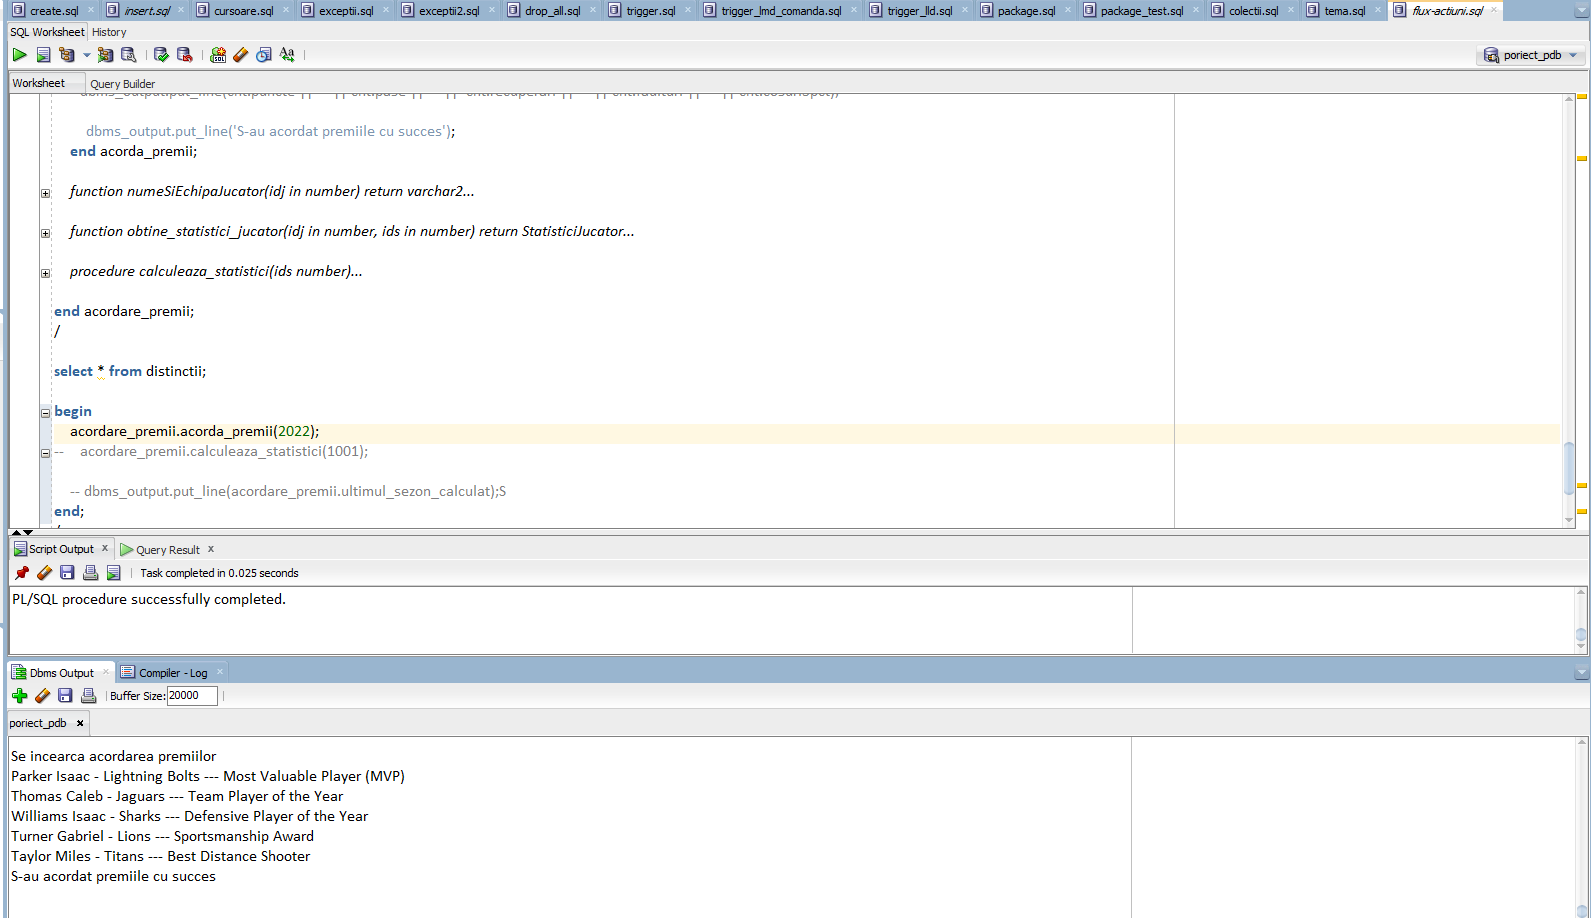
\includegraphics[width=40em, keepaspectratio]{flux-actiuni}
\pagebreak

\end{document}